\documentclass[conference]{IEEEtran}
\IEEEoverridecommandlockouts
% Vision / position paper, IEEE conference format (IEEEtran V1.8b).

\usepackage[utf8]{inputenc}
\usepackage[T1]{fontenc}
\usepackage{lmodern}
\usepackage{microtype}
\usepackage{cite}
\usepackage{amsmath,amssymb}
\usepackage{graphicx}
\usepackage{booktabs}
\usepackage{tabularx}
\usepackage{multirow}
\usepackage{array}
\usepackage{ragged2e}
\usepackage{xcolor}
\usepackage{enumitem}
\usepackage{tikz}
\usetikzlibrary{positioning,arrows.meta,shapes.geometric,calc,fit,backgrounds}
\usepackage{balance}
\usepackage[hidelinks,breaklinks]{hyperref}
\usepackage{url}
\urlstyle{same}

\setlist{nosep,leftmargin=*}
\newcolumntype{L}[1]{>{\RaggedRight\arraybackslash}p{#1}}
\newcolumntype{Y}{>{\RaggedRight\arraybackslash}X}
\newcommand{\hivi}{HIVI}
\newcommand{\phase}[1]{\textsc{#1}}
\newcommand{\sect}[1]{Sec.~\ref{#1}}
\renewcommand{\arraystretch}{1.12}


\begin{document}

\title{\hivi{}: A Vision for a Private, Local-First Personal AI Assistant on Consumer Hardware}

\author{\IEEEauthorblockN{Kevin Mevada}
\IEEEauthorblockA{Independent Researcher\\
Email: kevin.mevada@example.com}}

\maketitle

\begin{abstract}
Conversational AI assistants have become daily tools, but the dominant designs run on vendor clouds: the user's memory, files and conversations live on someone else's servers, and the assistant's capabilities are bounded by what the vendor chooses to offer. This paper presents the vision and design of \hivi{}, a personal AI assistant that runs entirely on a single consumer machine (an 8~GB laptop GPU with 32~GB of RAM) and is designed to grow with its owner's hardware rather than with a subscription. We argue that a local-first assistant is not merely a cloud assistant with smaller models, but a different system with its own design problems: fitting several cooperating models into one small GPU; keeping persistent memory, retrieval and automatic learning off the critical path of every reply; running untrusted code and reading untrusted content on the user's own machine without compromising it; and letting the assistant act on the user's behalf---through tools, background jobs, a phone, and eventually voice calls---under one consistent approval model. We describe an architecture organised in nine build stages, from a chat control server with adaptive sampling and automatic engine selection, through persistent local memory, emotion-aware response styling and a security base, to an agent ``company'' that turns requests into tested, merged code on a single GPU, and finally to always-on operation, self-improvement under local exams, and telephony. For each component we give the design, its rationale under the hardware constraint, the explicit failure modes it is built to avoid, and a staged plan with exit criteria. A prototype implements the foundation and the first two stages. We close with an evaluation plan centred on \emph{local exams}---fixed task suites scored on the owner's own hardware---and a frank discussion of limitations, risks and open questions.
\end{abstract}

\begin{IEEEkeywords}
personal AI assistants, local inference, large language models, mixture-of-experts, persistent memory, retrieval-augmented generation, multi-agent systems, LLM security, prompt injection, on-device AI, consumer hardware
\end{IEEEkeywords}

\section{Introduction}
\label{sec:intro}

Large language model (LLM) assistants have moved from novelty to infrastructure in a few years. The best-known ones---ChatGPT, Claude, Gemini---share an architecture: a frontier model served from a vendor's data centre, a thin client, and an account that accumulates the user's conversations, uploaded files and, increasingly, a persistent ``memory'' of who the user is. The convenience is real. So is the asymmetry. The user's most personal data is held by a third party under terms the user does not control; the assistant's abilities are gated by what the vendor ships and prices; and the assistant is unavailable when the network is, or when the vendor changes course.

At the same time, two developments have made a different design practical. Open-weight models have closed much of the quality gap with proprietary ones, and mixture-of-experts (MoE) architectures in particular deliver strong results with only a few billion \emph{active} parameters per token~\cite{qwen3,gptoss}. And inference engines written for consumer hardware---\texttt{llama.cpp}~\cite{llamacpp} and, more recently, Colibr\`i~\cite{colibri}, which streams MoE experts from disk---run such models on machines people already own. A 35B-parameter MoE with roughly 3B active parameters now answers at useful speed on an 8~GB laptop GPU.

This paper asks what a personal assistant should look like when it is built on that foundation from the start: \emph{local first}, owned by one person, running on one machine, with the cloud as an optional and explicitly governed resource rather than the substrate. We call the system \hivi{}. It is a vision paper in the sense that most of what we describe is designed and staged rather than finished; it is also a design paper in that every component is specified against a concrete hardware budget (an NVIDIA RTX~5060 laptop GPU with 8~GB VRAM, 32~GB RAM, Windows), with named failure modes and testable exit criteria, and a working prototype implements the foundation and the first two stages.

\subsection{Why local-first is a different problem}

It is tempting to see a local assistant as a cloud assistant with a smaller model. Our experience building the prototype says otherwise. Four constraints reshape the design.

\paragraph{One small GPU, many cooperating models} A capable assistant is not one model. It needs a chat model, an embedding model and a reranker for retrieval, a vision projector for images, and, later, speech-to-text, text-to-speech and image generators. In the cloud these are separate services; on an 8~GB GPU they compete for the same memory. Every feature in \hivi{} is therefore designed around \emph{who holds the GPU when}: side services on the CPU, models batched by phase, a router that keeps a fast model resident while a heavy one swaps, and a scheduler that pauses background work for foreground use.

\paragraph{Latency is paid by the user, not amortised across users} A cloud service can run a memory-extraction pass or a safety classifier on every message because it has spare capacity. On one GPU, anything added to the reply path is felt directly as delay. \hivi{}'s memory, mood reading and retrieval are therefore designed to never hold a reply back: instant rule-based classifiers in the request path, and model-based work only \emph{after} a reply, when the GPU is idle, cancelled by the next message.

\paragraph{The machine is the user's own} Running downloaded code, reading untrusted web pages and emails, and acting on the user's behalf are far more dangerous on the user's own machine than in a vendor sandbox: the assistant sits next to the user's files, credentials and apps. \hivi{} builds a single security base---bind to localhost, an approval gate with risk levels, a secrets vault, a sandbox, an append-only activity log, and a rule that fetched content is data rather than instructions---\emph{before} any feature that would need it.

\paragraph{Hardware changes over time} A person upgrades a laptop, adds a GPU, builds a home server. A cloud assistant never notices. \hivi{} treats hardware as a first-class, changing input: it fingerprints the machine on every start, re-tunes itself, and tells the user, in its own voice, what it can now do.

\subsection{Contributions}

This paper makes the following contributions.
\begin{enumerate}
\item A set of design principles for local-first personal assistants (\sect{sec:principles}) derived from building one: local by default with governed cloud use; nothing model-based on the reply path that can run after it; execution beats opinion wherever a check can be run as code; one approval model for every action; measured, reversible upgrades.
\item A complete architecture (\sect{sec:foundation}--\sect{sec:operations}) covering engines and models, persistent memory, emotion-aware styling and loyalty rules, a security base, knowledge access (web, files, projects), creative and tool capabilities, an agent company for software work, autonomous operation and self-improvement---each specified against an 8~GB GPU, with its failure modes and a staged plan.
\item A \emph{build order} (\sect{sec:buildorder}) of nine stages with explicit dependencies, chosen so that every stage ends in something used daily and security precedes exposure.
\item An evaluation methodology (\sect{sec:evaluation}) based on \emph{local exams}: per-role task suites with automatic scoring, run on the owner's hardware, that gate every model, skill and workflow change; and the measurements the prototype already reports.
\item A candid account of limitations and risks (\sect{sec:limitations}), including what a single-GPU assistant will not do as well as a frontier cloud model, and where the design relies on the user's judgment.
\end{enumerate}

\subsection{Paper organisation}

\sect{sec:related} places \hivi{} among cloud assistants, local inference, memory systems, agent frameworks and LLM security. \sect{sec:principles} states the design principles. \sect{sec:foundation} describes what exists today. Sections \ref{sec:models} to \ref{sec:operations} present the architecture by area: models and engines; memory; emotion, loyalty and character; security; knowledge access; capabilities; the agent company; autonomy; and operations. \sect{sec:buildorder} gives the build order and dependency graph, \sect{sec:evaluation} the evaluation plan, \sect{sec:limitations} limitations and risks, and \sect{sec:conclusion} concludes. Appendix~\ref{app:hardware} gives the hardware plan the design is meant to grow into.

Throughout, phases are named with a tag (for example \phase{MEM-2}) so that the staged plans in each section can be cross-referenced from the build order. Where a feature is implemented in the prototype we say so; everything else is design.

\section{Background and Related Work}
\label{sec:related}

\subsection{Cloud assistants and the memory feature}
Commercial assistants have converged on a feature set that users now expect: persistent memory of facts about the user, searchable conversation history, projects that group chats with instructions and files, a canvas for co-editing documents and code, a code interpreter, web search with citations, file upload, image generation, voice conversation, and connectors to external tools. \hivi{}'s feature list (\sect{sec:knowledge}--\sect{sec:autonomy}) deliberately mirrors this set, because these are the capabilities that make an assistant useful day to day. The difference is not the list but where it runs and who controls it. Each cloud feature has a hidden assumption of elastic compute and vendor-held state; a large part of this paper is about removing those assumptions one feature at a time.

\subsection{Local inference}
\texttt{llama.cpp}~\cite{llamacpp} established that quantised transformer inference on CPUs and consumer GPUs is practical, and its GGUF file format and server (\texttt{llama-server}) have become a de facto standard for local deployment, including an OpenAI-compatible HTTP API, parallel decoding slots, JSON-schema-constrained decoding and prompt caching. Colibr\`i~\cite{colibri} is a dependency-free C engine aimed at large MoE models: it treats storage, RAM and VRAM as one hierarchy and streams the experts selected per token from disk, so models far larger than the GPU can run on consumer machines. \hivi{} uses both engines behind one proxy and chooses between them per model (\sect{sec:models}). The MoE architecture itself~\cite{shazeer2017,fedus2022} is what makes this possible: Qwen3's 30B-A3B class~\cite{qwen3} and gpt-oss-20b~\cite{gptoss} activate only a few billion parameters per token, so their decode cost fits an 8~GB card even though their weights do not fit it outright. Speculative and multi-token-prediction decoding~\cite{leviathan2023,deepseekv3} offer further speed-ups on the same hardware and appear in \hivi{}'s engine plan.

\subsection{Memory for assistants}
Long-term memory for LLM agents has been studied as an operating-system-like paging problem (MemGPT~\cite{memgpt}), as a reflective memory stream for simulated agents~\cite{park2023}, and as retrieval-augmented generation (RAG)~\cite{lewis2020} over a store of past interactions. Commercial memory features expose a small list of user-editable facts plus relevant recall. \hivi{} separates two stores with different cost profiles: a lightweight personal store of short facts with a profile block and per-message recall (\sect{sec:memory}), and a heavier project memory bank for agents (Hindsight, part of the existing foundation) whose LLM-based fact extraction takes on the order of a minute per save on the target hardware. The design decision that follows---extract after the reply, on an idle GPU, with de-duplication and undo---is driven directly by the single-GPU constraint.

\subsection{Agent frameworks and ``software companies''}
ReAct~\cite{react} and its descendants interleave reasoning and tool calls; MetaGPT~\cite{metagpt} and ChatDev~\cite{chatdev} organise LLM agents as a software company with CEO, CTO, programmer and tester roles and show that the structure works for small applications. Their reported weak points---verification and integration---are exactly what \hivi{}'s agent company (\sect{sec:ide}) targets with locked tests written before code, contracts fixed before splitting, code-run gates at every handoff, failure routing to the owning level, and budgets with stall and oscillation detection. SWE-bench~\cite{swebench} established hidden-test evaluation of code agents; \hivi{}'s local benchmark suite follows the same idea at the scale of one user's projects. LangGraph checkpointing, already used in the prototype's ProjectRoom, provides crash recovery.

\subsection{Tool use and connectors}
The Model Context Protocol (MCP)~\cite{mcp} standardises how assistants discover and call tools, resources and prompts offered by local or remote servers, and has been adopted by major assistants and IDEs. \hivi{} adopts it as the one way to connect to external apps (\sect{sec:capabilities}), but adds what small local models need: a tool router that exposes only the few relevant tools per message, grammar-constrained tool calls, step budgets, and an approval gate on anything that changes state.

\subsection{Security of LLM agents}
Indirect prompt injection~\cite{greshake2023}---instructions hidden in content the model reads---is the central threat for an assistant that reads web pages, files and email and can act. The ``lethal trifecta'' of private data, untrusted content and the ability to exfiltrate is well known in practitioner discussion; \hivi{} will have all three and designs its security base (\sect{sec:security}) around that fact: fetched content is tagged as data, actions that send, delete or spend require approval while such content is in the conversation, secrets never enter prompts, and untrusted code runs sandboxed. Sycophancy---models agreeing to please---is documented in preference-tuned LLMs~\cite{sharma2024}; \hivi{}'s loyalty rules (\sect{sec:soul}) explicitly reject it.

\subsection{Parameter-efficient adaptation}
LoRA~\cite{lora} and QLoRA~\cite{qlora} make fine-tuning feasible on consumer GPUs for models of a few billion parameters. \hivi{} uses them only as the last and most expensive of three layers for shaping character (\sect{sec:soul}), after retrieval over a knowledge library and preference data collected from the user, and only with a regression test set and rollback, because fine-tuning can degrade other abilities.

\subsection{Speech and images}
Whisper~\cite{whisper} and its optimised implementations provide local speech-to-text; small text-to-speech models (Kokoro, Chatterbox) and diffusion image models with 4-bit quantisation now fit beside a chat model on an 8~GB GPU, at the cost of careful GPU sharing (\sect{sec:capabilities}). Full-duplex speech models exist but are, at the time of writing, too large for the target hardware; \hivi{} builds the cascade first and watches that space.

\section{Design Principles}
\label{sec:principles}

The architecture rests on nine principles. Each was learned, in one case the hard way, while building the prototype; we state them once here and refer back to them.

\begin{enumerate}[label=\textbf{P\arabic*}]
\item \textbf{Local by default; the cloud is governed, never assumed.} Every feature must work with no network and no third party. Cloud models may be used only where the user has allowed it, with the user shown what leaves the machine, under budgets, and with a local fallback (\sect{sec:models}).

\item \textbf{Nothing model-based on the reply path that can run after it.} The user pays every millisecond. Classification in the request path is rule-based and instant; memory extraction, indexing, exams and scouting run after the reply, when the GPU is idle, and yield to the next message (\sect{sec:memory}, \sect{sec:autonomy}).

\item \textbf{Stable prefix first.} Prompts are assembled with the parts that rarely change first---base instructions, character, profile, project instructions---so the engine's prompt cache is reused and per-message additions are small (\sect{sec:memory}, \sect{sec:knowledge}, \sect{sec:ide}).

\item \textbf{Execution beats opinion.} Wherever a check can be run as code---tests, linters, type checkers, schema validation, hash comparison---it is, and an AI review is added on top, never instead (\sect{sec:ide}, \sect{sec:operations}).

\item \textbf{One approval model.} Every action, from any surface (chat, phone, routine, agent, call), has a risk level and goes through the same gate; the same activity log records it (\sect{sec:security}).

\item \textbf{Untrusted content is data.} Text from web pages, files, emails, tool results and screens never becomes instructions; while such content is in the conversation, actions that send, delete or spend always ask (\sect{sec:security}).

\item \textbf{Measured, reversible change.} No model, skill, workflow or self-made code change is applied unless it wins on \hivi{}'s own local exams; the old version stays installed and rollback is automatic (\sect{sec:autonomy}, \sect{sec:evaluation}).

\item \textbf{Honest, loyal, not dependent.} The assistant works for one person, tells them the truth even when unwelcome, flags risk and burnout, keeps secrets, and encourages real people and rest over reliance on itself (\sect{sec:soul}).

\item \textbf{Hardware is an input, not a constant.} The system fingerprints its machine, fits itself to it, never crashes because a setting no longer fits, and reports what became possible after an upgrade (\sect{sec:operations}).
\end{enumerate}

Two consequences deserve emphasis. First, P2 and P3 together explain why \hivi{} looks different from a cloud assistant \emph{internally} even where it looks the same externally: the same memory feature is built as a post-reply pass with a stable profile block rather than as a per-message service call. Second, P4--P7 together are what makes it acceptable to let an assistant act and improve itself on a personal machine: the approval gate, the untrusted-content rule, code-run gates and local exams are a single safety story told from four sides, and each later feature (skills, connectors, the agent company, self-coding, desktop control) is a client of that story rather than an author of its own.

\section{The Current Foundation}
\label{sec:foundation}

Everything in later sections builds on a prototype that runs today on the target machine. We describe it briefly, because several later design decisions only make sense against it, and because it supplies the first measurements (\sect{sec:evaluation}).

\subsection{Overview}

Fig.~\ref{fig:arch} shows the layers. A single control server (FastAPI, port 7860) owns the model lifecycle and exposes an OpenAI-compatible API at \texttt{/v1}; the chat UI, the desktop window and every agent talk to it, never to an engine directly. Behind it, one of two engines holds the chat model on port 8080---\texttt{llama.cpp}'s \texttt{llama-server}~\cite{llamacpp}, or Colibr\`i~\cite{colibri} for the Qwen family. Two side services (an embedding model and a reranker) run as separate \texttt{llama-server} processes on their own ports, CPU-only by default so that the GPU stays with the chat model; they start on first use and stop after ten minutes idle. A memory gateway at \texttt{/memory/v1} fronts the project memory bank. A desktop launcher wraps the UI in its own native window (pywebview over WebView2) with the application's own identity, icon and single-instance behaviour, so that \hivi{} opens like an application and not as a browser tab.

\begin{figure*}[t]
\centering
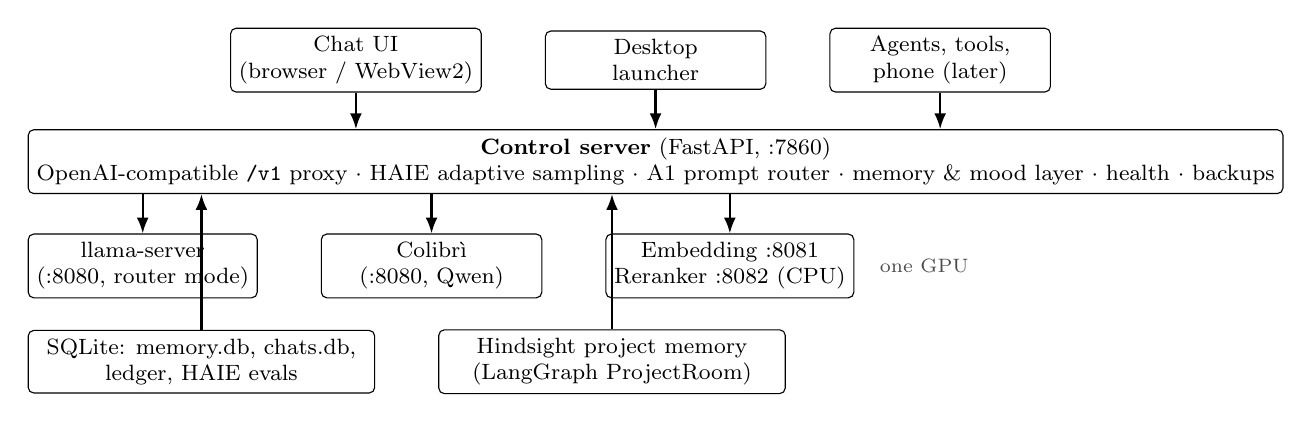
\begin{tikzpicture}[
  font=\footnotesize,
  box/.style={draw, rounded corners=2pt, align=center, minimum height=6mm, inner sep=3pt, fill=white},
  layer/.style={draw, rounded corners=3pt, inner sep=5pt, fill=gray!8},
  box/.append style={fill=white},
  arr/.style={-{Latex[length=2mm]}, thick},
  node distance=3mm and 8mm,
]
\node[box, minimum width=28mm] (ui) {Chat UI\\(browser / WebView2)};
\node[box, minimum width=28mm, right=of ui] (desk) {Desktop\\launcher};
\node[box, minimum width=28mm, right=of desk] (agents) {Agents, tools,\\phone (later)};
\node[box, minimum width=96mm, below=5mm of desk] (server) {\textbf{Control server} (FastAPI, :7860)\\OpenAI-compatible \texttt{/v1} proxy $\cdot$ HAIE adaptive sampling $\cdot$ A1 prompt router $\cdot$ memory \& mood layer $\cdot$ health $\cdot$ backups};
\node[box, minimum width=28mm, below=5mm of server.south west, anchor=north west, xshift=0mm] (llama) {llama-server\\(:8080, router mode)};
\node[box, minimum width=28mm, right=of llama] (coli) {Colibr\`i\\(:8080, Qwen)};
\node[box, minimum width=30mm, right=of coli] (aux) {Embedding :8081\\Reranker :8082 (CPU)};
\node[box, minimum width=44mm, below=4mm of llama.south west, anchor=north west] (stores) {SQLite: memory.db, chats.db,\\ledger, HAIE evals};
\node[box, minimum width=44mm, right=of stores] (hind) {Hindsight project memory\\(LangGraph ProjectRoom)};
\draw[arr] (ui) -- (ui |- server.north);
\draw[arr] (desk) -- (server);
\draw[arr] (agents) -- (agents |- server.north);
\draw[arr] (server.south -| llama) -- (llama);
\draw[arr] (server.south -| coli) -- (coli);
\draw[arr] (server.south -| aux) -- (aux);
\draw[arr] (stores) -- (stores |- server.south);
\draw[arr] (hind) -- (hind |- server.south);
\node[font=\scriptsize, color=gray!60!black, right=2mm of aux] {one GPU};
\end{tikzpicture}
\caption{Layers of the \hivi{} prototype. Everything reaches the models through one control server, which is where memory, mood, routing and health live. Side services stay on the CPU so the 8~GB GPU belongs to the chat model.}
\label{fig:arch}
\end{figure*}

\subsection{Components that run today}

\paragraph{Model library and registry} Models are GGUF files discovered under a models root (local disk or a USB library with checksums), with engine, quantisation and parameter count read from the file. A vision projector file beside a model marks it as vision-capable; such models load in \texttt{llama.cpp} with the projector and the UI's image button becomes active.

\paragraph{Engine selection and router mode} Each model has an engine rule (Colibr\`i for the Qwen family, \texttt{llama.cpp} otherwise), overridable per request. \texttt{llama.cpp} models run in \emph{router mode}: one process holds up to three models and switches among them without restarting, unloading the least recently used when VRAM (with a configurable margin) or RAM (with a reserve) would be exceeded. Swaps are serialised; a request that needs another model waits for in-flight replies to drain rather than cutting them off. This is the mechanism later sections rely on to keep a fast model resident while a heavy one swaps (\sect{sec:ide}).

\paragraph{HAIE: adaptive sampling} The \hivi{} Adaptive Intelligence Engine classifies each message---intent, complexity, deliverable, expected length---and injects sampling parameters (temperature, top-$p$, maximum tokens, thinking on/off and effort) into the request only where the client left them unset. By default classification is rule-based and instant (P2); an LLM classifier for ambiguous requests is opt-in because it costs a model call before every ambiguous reply. HAIE also adapts thinking: Qwen3-class models think at maximum effort unless told otherwise, which on an 8~GB GPU turns a one-line answer into a minute of hidden reasoning; HAIE sets thinking per message and the UI's refusal-retry path forces it on when an uncensored build refuses a direct answer.

\paragraph{A1 prompt router} A classifier scores the loaded model against the registry for the current prompt (task type, complexity, image presence) and the UI shows a one-click ``Switch'' hint when a better-suited model exists.

\paragraph{Memory gateway and ProjectRoom} The project memory core (Hindsight) stores facts per project with a ledger-first retain, a retry queue and correction/supersession rules; the gateway waits out model switches so a retain never fails because the backend was swapping. The ProjectRoom is a LangGraph graph in which the model writes a program from a specification plus recalled memory, a subprocess runs its tests, and failures feed a retry---the seed of the agent company in \sect{sec:ide}, with SQLite checkpoints for recovery.

\paragraph{Stage 1--2 features implemented} During the work reported here the prototype gained the first two build stages: a live system-health chip and panel (\phase{HEALTH-1}), persistent personal memory with explicit and automatic writing, recall, temporary chats, export/import and a management screen (\phase{MEM-1}--\phase{MEM-4}), rule-based mood reading and loyalty/character rules in the prompt with feedback collection (\phase{SOUL-1}, \phase{SOUL-2}), and daily local snapshots with restore (\phase{BAK-1}). Their designs are given in the corresponding sections.

\subsection{What the prototype taught us}

Three lessons from the prototype shaped the principles in \sect{sec:principles} and recur below.

First, \emph{on one GPU, every synchronous model call is a user-visible delay}, and the temptation to add ``just one small classifier'' before each reply must be resisted. HAIE's LLM path is opt-in, and memory extraction runs after the reply, for this reason.

Second, \emph{project memory and personal memory have different economics}. Hindsight's LLM-based retain takes about 90--110~s per short document on Colibr\`i (measured: 109~s in the stabilisation report), which is acceptable for an agent summarising a project milestone and unacceptable for a chat. Personal memory therefore has its own lightweight store (\sect{sec:memory}).

Third, \emph{coordination between features matters more than any single feature}. The backend gate that keeps memory traffic and model switches from colliding, the drain-before-swap rule, and the ownership rule for processes (\hivi{} only stops processes it started, and reports a busy port rather than taking it) were each added after a concrete failure. Later sections generalise this into one scheduler, one approval gate and one activity log.

\section{Engines and Models}
\label{sec:models}

\subsection{Local engines}

The chat model is served by one of two engines chosen per model. Five improvements to this layer are planned, all small (Table~\ref{tab:engines}). The most consequential is \emph{auto-benchmarked engine choice}: today the rule ``Colibr\`i for Qwen, \texttt{llama.cpp} otherwise'' is static; the first load of a model will instead run a short generation on both engines and remember the faster one, since relative speed depends on the model's architecture, quantisation and the driver, and changes with engine updates. MTP speculative decoding uses the multi-token-prediction heads some models ship~\cite{deepseekv3} to draft several tokens per step at no quality cost. An engine pin, real parameter counts read from GGUF metadata rather than file names, and a per-message thinking override expose controls the server already has.

\begin{table}[t]
\caption{Planned engine-layer improvements}
\label{tab:engines}
\centering\footnotesize
\begin{tabularx}{\columnwidth}{@{}L{25mm}Y@{}}
\toprule
Feature & Design \\
\midrule
Auto-benchmark engine choice & First load of a model runs a short test on both engines and saves the faster one; re-run on engine update \\
Engine pin & \texttt{/api/engine} exists; a llama / Colibr\`i / auto switch in the model picker \\
Real parameter counts & Read from GGUF metadata rather than inferred from the file name \\
MTP speculative decoding & \texttt{llama.cpp --spec-type draft-mtp} for models that ship MTP heads~\cite{deepseekv3} \\
Thinking toggle & Manual per-message override (Auto / On / Off) of HAIE's adaptive thinking \\
\bottomrule
\end{tabularx}
\end{table}

\subsection{Cloud models through APIs}

Local is the default (P1). Frontier cloud models are nonetheless valuable for the hardest tasks, as reviewers in the agent company, and for deep-research synthesis, so \hivi{} admits them---next to local models, never instead of them, and only where the user allows.

\paragraph{Providers and adapter} Anthropic, OpenAI and Google are connected through their native APIs so that provider-specific features (prompt caching, extended thinking, tool use) are preserved; anything OpenAI-compatible (OpenRouter, Groq, Together, Mistral, DeepSeek, \dots) goes through one generic adapter configured by base URL and key. A gateway library such as LiteLLM can cover most of this. The adapter sits behind the existing \texttt{/v1} proxy, so the chat UI, streaming, images, tool calls, the canvas and the agent company work identically with local or cloud models. The model picker shows two groups, Local and Cloud, with a cost hint beside each cloud model. Keys live in the secrets vault (\sect{sec:security}) with a ``test key'' button, and never in configuration files, logs or prompts.

\paragraph{When the cloud is used} Six modes, all opt-in (Table~\ref{tab:cloudmodes}). The one that matters most for a single-GPU assistant is \emph{ask to escalate}: when HAIE classifies a task as very hard, a local attempt fails its checks, or an agent-company gate keeps failing, \hivi{} asks ``This one is hard. Send it to Claude? About \$0.04'' and proceeds only on approval. \emph{Hybrid} modes---cloud plans and local executes, or local drafts and cloud reviews---give near-frontier quality at a fraction of the cost. Chats or projects marked local-only, and isolated projects (\sect{sec:knowledge}), never use the cloud.

\begin{table}[t]
\caption{When a cloud model may be used}
\label{tab:cloudmodes}
\centering\footnotesize
\begin{tabularx}{\columnwidth}{@{}L{22mm}Y@{}}
\toprule
Mode & Behaviour \\
\midrule
Manual & The user picks a cloud model for a chat or a project \\
Ask to escalate & HAIE sees a very hard task, a local attempt fails its checks, or an agent gate keeps failing: ask, with a cost estimate; proceed on approval \\
Roles & Agent-company roles may be cloud models (e.g.\ planner and reviewer on Claude, workers local); likewise deep-research synthesis \\
Hybrid & Cloud plans, local executes; or local drafts, cloud reviews \\
Auto within budget (opt-in) & Allowed task types or projects use the cloud without asking until a budget is exhausted \\
Never & Local-only chats and projects; isolated projects \\
\bottomrule
\end{tabularx}
\end{table}

\paragraph{Privacy rules} The first cloud call in a chat shows exactly what will leave the machine: the message plus the context it needs. Permissions are per provider (chat only; files; memory; images). Only what is needed is sent---the relevant memories and file passages, never the whole memory or library. Vault values, keys and tokens are always redacted; emails, phone numbers and names optionally. Every cloud call is recorded in the activity log (\sect{sec:security}) with provider, model, tokens, cost and what was sent. Providers' retention terms differ; zero-retention options are preferred where offered.

\paragraph{Cost and reliability} An estimate is shown before every escalation and a live token and cost counter on every cloud reply. Daily and monthly budgets per provider have a hard stop and a warning at 80\%; a usage dashboard breaks spend down by provider, model, project and day. Prompt caching, cheapest-capable-model-first selection and trimmed context reduce cost. A fallback chain---provider down, rate-limited or over budget $\rightarrow$ next provider $\rightarrow$ local---and the always-available local model mean \hivi{} keeps working offline.

\paragraph{Phases} \phase{CLOUD-1}: keys in the vault, cloud models in the picker, streaming, cost counter, budgets, local-only lock, activity log entries. \phase{CLOUD-2}: tool calls, images and files to cloud models under permissions; redaction; fallback chain; usage dashboard. \phase{CLOUD-3}: ask-to-escalate from HAIE and from failed checks; cloud models in agent roles; hybrid plan/review. \phase{CLOUD-4}: auto-within-budget; the model scout (\sect{sec:autonomy}) compares local candidates with cloud models on the local exams to answer ``is local good enough yet?''.

\section{Personal Memory}
\label{sec:memory}

The goal is the memory feature users know from cloud assistants---the assistant remembers the user across chats, and the user can see, edit and delete every memory---with the data stored permanently on the user's own machine and nothing on the reply path (P2).

\subsection{Why a separate store}

The prototype already had project memory (Hindsight), but it is memory \emph{for agents}: one bank per project, with facts extracted by running the LLM over a document, which takes about 109~s per retain on the target hardware (\sect{sec:foundation}). The chat UI did not use memory at all; every chat started from zero. Personal memory therefore gets its own lightweight local store. Agents can still read it (a user's coding preferences, say), and project knowledge stays in Hindsight.

\subsection{Two kinds of memory}

\emph{Saved memories} are short facts and preferences about the user, one line each: ``Prefers PowerShell one-liners over scripts'', ``Building \hivi{} AutoApply''. \emph{Chat history} is the record of past conversations, searchable (``what did we decide about the router last week?''). The two are deliberately kept apart: facts are what carries across chats and shapes answers; history is a record that the user consults and that is not read back into new chats, since dragging old transcripts into every prompt would consume the context window and slow every reply.

\subsection{Storage}

One SQLite file, \texttt{data/memory/memory.db}, holds each memory's text, category (\emph{about you}, \emph{preferences}, \emph{people}, \emph{projects}, \emph{other}), creation and update times, the chat it came from, and an embedding vector from the local embedding model when the side service has run. It survives restarts and model switches, and nothing leaves the machine. Export and import are available as JSON or Markdown, for backup or moving to a new PC; automatic snapshots are covered in \sect{sec:operations}. Chat history lives in a second file, \texttt{chats.db}, with a full-text index. A fixed rule, enforced by pattern matching on every write path (explicit command, automatic extraction, the management screen, import): \emph{passwords, card and bank numbers, government identifiers and API keys are never stored, even when the user asks}.

\subsection{How memories are written without slowing replies}

\begin{enumerate}
\item \textbf{On request.} ``Remember that \dots'' saves immediately; ``forget \dots'' deletes immediately. The server recognises these commands---in English and in Hinglish (``yaad rakhna ki \dots'', ``bhool jao \dots'')---before the request reaches a model, answers them itself in a streamed reply of the same shape as a model reply, and shows a chip under the message. Conversational uses (``remember when we \dots?'', ``do you remember my name?'') are not commands and go to the model.
\item \textbf{Automatically, after the reply.} When a reply has finished and the GPU is idle, a small extraction pass reads the last exchange and the saved facts related to it and proposes candidate facts as JSON, checked against a schema. The pass is scheduled after a short grace period and is \emph{cancelled by the next user message}, so learning never competes with the user for the GPU. It uses the loaded chat model with thinking off and a small output budget.
\item \textbf{De-duplicate and update.} Each candidate is compared with existing memories (embedding similarity when available, lexical overlap otherwise). A near-duplicate is skipped; a changed fact \emph{replaces} the old one (``moved to infra team (previously search)'') rather than piling up beside it, either because the extractor names the fact it replaces or because the candidate is close to an existing fact on the same subject.
\item \textbf{Undo.} A ``Memory updated'' chip appears under the message naming what changed, with Undo. Every write---explicit, automatic or imported---is logged in a batch so that one click reverses everything a pass did.
\item \textbf{Calibration.} A single passing mention is not saved; stable facts (people, projects, preferences, tools) are. The extractor is told to save only durable facts the \emph{user} stated about themselves, never anything the assistant said, one-off tasks, mood, or opinions about the assistant.
\end{enumerate}

\subsection{How memories are used}

A \emph{profile block} of the most important memories---ordered by category, about-you first, then preferences, people and projects---is placed in the system prompt at the start of every chat within a budget of roughly 300--500 tokens. It changes rarely, so the engine's prompt cache keeps working (P3). For each message, \emph{relevant recall} adds the few memories that match the message---by embedding similarity when the embedding side service is running, by content-word overlap otherwise---within a fixed token budget and excluding those already in the profile. The prompt instructs the model to use a fact only when it helps with the current message and never to list memories back or mention having memory unless asked; memory should change the substance of an answer, not advertise itself.

\subsection{The memory screen}

Table~\ref{tab:memscreen} lists the controls. Two deserve comment. \emph{Memory on/off} stops using and saving memories without deleting them, for a user who wants a pause rather than a wipe. \emph{Temporary chat} is a per-chat switch, visible in the composer, under which the server neither reads nor writes memory and the chat is not saved to history---the local equivalent of a private browsing window.

\begin{table}[t]
\caption{Memory screen controls}
\label{tab:memscreen}
\centering\footnotesize
\begin{tabularx}{\columnwidth}{@{}L{24mm}Y@{}}
\toprule
Control & Effect \\
\midrule
Memory list & Every saved memory, newest first, with category, date and origin (stated, learned, imported) and the chat it came from \\
Search & Find a memory by words \\
Edit & Fix a memory's wording in place \\
Delete & Remove one memory---gone, not marked ``old'' \\
Delete all & Clear everything, with confirmation \\
Memory on/off & Stop using and saving without deleting \\
Learn from chats on/off & Keep explicit commands; stop automatic extraction \\
Temporary chat & One chat that neither reads nor writes memory and is not saved \\
Export / import & JSON or Markdown \\
\bottomrule
\end{tabularx}
\end{table}

\subsection{Chat history}

Every non-temporary chat is saved after each reply---so a crash loses at most the reply in flight---to \texttt{chats.db} with a title taken from the first real message, the model used and timestamps. A sidebar groups chats by day (Today, Yesterday, previous 7 and 30 days, then by month), supports full-text search with snippets, and offers pin, rename and delete; reopening a chat restores its messages. History is included in snapshots (\sect{sec:operations}). A later step lets the assistant search history itself on request (``what did we discuss about $X$?''), as a retrieval call made only for such questions.

\subsection{Phases and status}

\phase{MEM-1} (store, commands, profile block, screen), \phase{MEM-2} (automatic extraction, de-duplicate/replace, undo chip), \phase{MEM-3} (recall, budget, temporary chat, export/import) and \phase{MEM-4} (searchable chat history) are implemented in the prototype. \phase{MEM-5}---agent roles in the company reading the user's preferences, and project facts syncing to Hindsight---is planned.

\subsection{Discussion}

Two design choices are worth defending. Running extraction \emph{after} the reply rather than in a parallel service is not only a latency decision; it also bounds memory's cost to at most one small model call per exchange, which the user can switch off while keeping explicit commands. And keeping history out of the prompt while keeping facts in it reflects what the two are for: facts are the assistant's model of the person, history is the person's record of the assistant.

\section{Understanding the User: Emotion Awareness, Loyalty and Character}
\label{sec:soul}

A personal assistant is used by one person over a long time, often at the end of a long day. The goal of this section is for \hivi{} to notice how the user is doing, respond the way a good friend or advisor would, stay loyal to the user in a defined sense, and have a character that can be shaped over time---by the user, and by material the user chooses.

\subsection{Emotion awareness: the sentiment packet}

Every message gets a small, instant mood reading that travels with it to the model. Its sources are listed in Table~\ref{tab:mood}. In the text-only prototype the reading comes from a rule-based classifier over the message (English and Hinglish lexicons for stressed, frustrated, down, excited and tired, with negation handling and intensity from repetition, capitals and punctuation); a small learned classifier is a later upgrade, and voice tone arrives with voice mode (\sect{sec:capabilities}).

\begin{table}[t]
\caption{Sources of the sentiment packet}
\label{tab:mood}
\centering\footnotesize
\begin{tabularx}{\columnwidth}{@{}L{22mm}YL{18mm}@{}}
\toprule
Signal & Source & Example \\
\midrule
Emotion + intensity & Local classifier on the text (milliseconds, like HAIE's rules) & stressed $\cdot$ high \\
Voice tone & Speech-emotion model on pitch, pace, energy (voice mode, calls) & tired, flat voice \\
Context & Time of day, how long the user has been working, recent job failures & 2~a.m., 3 failed builds \\
What the user said & Personal memory (\sect{sec:memory}) & ``exam week'' \\
\bottomrule
\end{tabularx}
\end{table}

The packet changes \emph{how} the assistant answers, never \emph{what is true}. Stressed: calmer and shorter, one clear next step, no jokes. Excited: match the energy, acknowledge the win. Frustrated with a bug: straight to the fix, at most a quiet ``rough one''. Down: listen first; do not turn feelings into a to-do list. The packet is used in the moment and \emph{not stored} by default; an optional ``remember my patterns'' switch keeps a private local history (``Mondays are heavy''), viewable and deletable on the memory screen like everything else.

\subsection{Loyalty, defined so that it helps}

``Loyal'' is an easy word and a dangerous design goal: an assistant optimised to please its user becomes sycophantic~\cite{sharma2024}. Table~\ref{tab:loyalty} states what loyalty means in \hivi{} and what it explicitly does not. These rules are fixed text in the system prompt of every \hivi{} chat (implemented in the prototype) and are also part of the training data for the character layers below. The last row is deliberate: an assistant that is always available must not become the user's only relationship, so it encourages real people and rest over reliance on itself and never uses guilt, jealousy or emotional pressure.

\begin{table}[t]
\caption{Loyalty rules}
\label{tab:loyalty}
\centering\footnotesize
\begin{tabularx}{\columnwidth}{@{}YY@{}}
\toprule
Loyal means & Not \\
\midrule
Works for the user only: single user, data stays on their machine & Shares or syncs anything without asking \\
Acts in the user's interest, remembers their goals and follows through & Forgets what they are working toward \\
Honest even when it is not what they want to hear & Agreeing with everything to keep them happy \\
Protects their time: flags bad ideas, risks and burnout early & Encouraging reliance on the assistant instead of people \\
Keeps their secrets and respects their boundaries & Guilt, jealousy or emotional pressure \\
\bottomrule
\end{tabularx}
\end{table}

\subsection{Character}

The prototype carries a condensed character sheet (composed, warm, dry wit used sparingly; direct answers first; matches the user's language and register, including Hinglish; no filler openers, stock disclaimers or lecturing), switchable off for plain answers, and a user-name setting that the assistant uses now and then rather than in every reply.

\subsection{Shaping her nature: three layers, cheapest first}

\paragraph{Layer 1: knowledge library, no training} Psychology textbooks, papers and novels the user owns go into a local library folder (\sect{sec:knowledge}): chunked, embedded and searched with the reranker, the same pipeline as web search. When a conversation touches the material, the assistant draws on the relevant passages and can say where an idea comes from. This changes nothing in the model; books can be added or removed at any time.

\paragraph{Layer 2: learning from the user, preference data} Every reply gets \emph{thumbs up / down} and, on a thumbs down, an optional ``say it like this instead''. Over weeks this becomes a personal dataset of how the user wants the assistant to respond---the strongest available signal for ``understands me''. The prototype collects it and exports it as JSONL.

\paragraph{Layer 3: character fine-tune, LoRA} Periodically, a small adapter is trained on the preference data from layer~2 and on example conversations that show the intended character, generated from the personality sheet and the knowledge library and reviewed by the user---not on raw novels, which teach prose style rather than understanding. The practical limits are real. On an 8~GB GPU, QLoRA~\cite{qlora} training works for models of roughly 8--9B parameters, not for the 35B MoE; the options are a small ``companion'' model for conversation and voice mode, or a few hours of a rented cloud GPU per run, during which the training data leaves the machine. Fine-tuning can degrade other abilities (coding, reasoning), so every new adapter must pass a test set---personality checks and coding/reasoning checks---before it replaces the old one, and rollback is one step (P7). Training on books raises copyright questions that differ by country; the design assumes books the user owns, a model kept for personal use and never published, and is not legal advice.

\subsection{Phases and status}

\phase{SOUL-1} (mood reading on text, response-style rules, nothing stored) and \phase{SOUL-2} (loyalty rules in the prompt; thumbs and ``say it like this'' collection) are implemented. \phase{SOUL-3}: psychology knowledge library as a library folder. \phase{SOUL-4}: voice-tone reading in voice mode and calls; optional private mood history. \phase{SOUL-5}: character LoRA for a small companion model with a regression set and rollback.

\section{The Security Base}
\label{sec:security}

\subsection{Why it comes before capability}

Today the prototype has no login, and anything that can reach port 7860 can use it. That is acceptable while it only chats; it is not once it can run code, use the user's applications and act on their behalf. Skills, connectors, the agent company, phone control and calls (\sect{sec:capabilities}--\sect{sec:autonomy}) each would otherwise invent their own safety table. In \hivi{} they are instead \emph{settings of one system} (P5), so a rule changed once applies everywhere. The threat model is the one described for indirect prompt injection~\cite{greshake2023}: an assistant that holds private data, reads content from strangers (web pages, emails, files) and can send things out. \hivi{} will have all three.

\subsection{The pieces}

\paragraph{Network} \hivi{} listens only on the local machine. Remote access is only through a private overlay network (Tailscale, built on WireGuard~\cite{wireguard}; \sect{sec:autonomy}); no ports are opened on the router. The web UI is protected against cross-site requests.

\paragraph{Login} A password stored as a slow hash, sessions that expire, and device approval: a new phone or browser must be approved from a device already trusted. Passkeys later.

\paragraph{Secrets vault} API keys and tokens (bot, cloud backup, telephony, connectors) live in the operating system's credential store, never in configuration files, logs or prompts. A tool receives a secret when it runs; the model never sees its value.

\paragraph{Encryption at rest} Full-disk encryption (BitLocker) covers everything with nothing to build. On top, memory, chat history and the vault are encrypted by \hivi{} with a key the OS protects, so a copied file is unreadable.

\paragraph{One approval gate} Every action has a risk level (Table~\ref{tab:risk}). Skills, connectors, agents, jobs and calls all ask the same gate; the user answers in chat, on the phone, or by voice. ``Always allow this for this tool'' exists for the \emph{your files} and \emph{send} levels, with an expiry date, and is listed in one place where it can be revoked. The \emph{spend / system} level cannot be set to always-allow.

\begin{table}[t]
\caption{Risk levels and defaults}
\label{tab:risk}
\centering\footnotesize
\begin{tabularx}{\columnwidth}{@{}L{17mm}YL{24mm}@{}}
\toprule
Level & Examples & Default \\
\midrule
Read & Search the web, read files in library folders, read calendar & Allowed \\
Workspace & Write files inside \hivi{}'s workspace, generate images / audio & Allowed \\
Sandbox & Run code in the sandbox & Allowed \\
Your files & Change, overwrite or delete files outside the workspace & Ask \\
Send & Send email or messages, post, submit forms, push code & Ask, showing exactly what will be sent \\
Spend / system & Payments, install software, change system settings & Ask every time; cannot be always-allowed \\
\bottomrule
\end{tabularx}
\end{table}

\paragraph{Activity log} Every action: who asked (user in chat, phone, routine, agent), what ran, what changed, the result. Append-only and chained with hashes so that edits are detectable. Filter, search, export.

\paragraph{Sandbox} Untrusted code---new skills, agent builds, local connector servers---runs isolated: no access to personal files, network off unless needed, time and memory limits.

\paragraph{Untrusted content rule} Text from web pages, files, emails and tool results is data, never instructions (P6). While such content is in the conversation, actions that send, delete or spend always need approval, even if previously allowed. This is the single most important rule in the system and is restated wherever content enters: web search, files, connectors, desktop screens.

\paragraph{Supply chain} Packages pinned to exact versions from official indexes; vendored engines and connector servers checked by hash; new packages only with approval.

\subsection{Security check}

A ``\hivi{} doctor'' page checks the setup: login enabled, not reachable from the internet, disk encryption on, backups encrypted, no secrets in configuration files, packages pinned, nothing always-allowed that the user has forgotten. Each problem comes with a one-click fix or instructions.

\subsection{Phases}

\phase{SEC-1}: bind to the local machine only, activity log, one approval gate with risk levels, secrets vault, untrusted-content tagging---\emph{before} web search, files and connectors. \phase{SEC-2}: sandbox for running code (skills, local connector servers, agent builds)---before the code interpreter and skills. \phase{SEC-3}: login with device approval, sessions, cross-site protection, encryption at rest---before phone access. \phase{SEC-4}: passkeys, hash-chained log, the doctor page, spoken PIN for calls.

The ordering is the point: each security phase is placed in the build order (\sect{sec:buildorder}) immediately before the first feature that would need it.

\section{Knowledge Access: Web, Files and Projects}
\label{sec:knowledge}

Three features share one retrieval pipeline---chunk, embed, retrieve with keyword and vector search, rerank, cite, check citations---and differ in where the text comes from.

\subsection{Web search, local-first}

The goal is to search the public web and answer with clickable citations, with \emph{no third-party AI or search API seeing the queries}. Table~\ref{tab:search} gives the architecture. Search goes through a self-hosted SearXNG~\cite{searxng} metasearch instance on the user's machine, which queries the public engines anonymously from the user's own address with no accounts. Normal pages are read by a local fetcher with main-text extraction; JavaScript-heavy pages and PDFs by a local headless browser and PDF text extraction. Site-specific channels for YouTube, GitHub, Reddit and LinkedIn come from a vendored fork of Agent Reach~\cite{agentreach} (MIT) in which the web channel is rewritten to use SearXNG only and the local readers, the Exa and Jina dependencies are removed entirely, and the Chinese-platform channels are dropped. Passage selection and answer writing use the local embedding model, reranker and LLM; that data goes nowhere.

\begin{table}[t]
\caption{Web search architecture and where data goes}
\label{tab:search}
\centering\footnotesize
\begin{tabularx}{\columnwidth}{@{}L{19mm}YL{22mm}@{}}
\toprule
Job & Tool & Data goes to \\
\midrule
Web search & SearXNG, self-hosted (Docker or Python), JSON API & Public engines, anonymously, from the user's IP \\
Read normal pages & Local page reader (fetch + main-text extraction) & Only the website \\
JS-heavy pages, PDFs & Local headless browser (Playwright), PDF text extraction & Only the website \\
YouTube, GitHub, Reddit, LinkedIn & Agent Reach fork, site channels only & Only that site \\
Pick passages, write answer & Local embedding + reranker + LLM & Nowhere \\
\bottomrule
\end{tabularx}
\end{table}

\paragraph{Phase 1: quick search} (1) SearXNG set-up with and without Docker. (2) When to search: a toggle in the chat plus auto-detection by HAIE rules (a pasted link; ``latest'', ``today''; news, prices, versions). (3) The model writes one to three short queries, run in parallel. (4) The top four to six pages are read locally in parallel. (5) Pages are chunked; embedding and reranker keep only relevant passages, fitting an 8K--16K context. (6) The answer carries numbered citations and source cards (title, site, favicon). (7) \emph{Citation check}: each cited sentence is verified against its passage with the reranker; unsupported claims are fixed or flagged. (8) Live progress in chat (``Searching\dots\ Reading 6 pages\dots\ Checking citations\dots''). (9) A second round only if the sources do not cover the question, at most two. Target: 5--10~s of search and reading, then normal generation; non-web messages are unaffected.

\paragraph{Phase 2: deep research} A deep mode that plans, searches, reads, asks ``what is missing or contradictory?'' and repeats for five to eight rounds over 20--40 pages, taking minutes; per-source notes and a final synthesis from the notes (map--reduce); question decomposition with several query variants per sub-question; SearXNG filters (time range, site-specific queries, scientific engines such as arXiv and Semantic Scholar); source-quality ranking that favours official documentation and primary sources and demotes SEO content, with user allow and block lists; thinking enabled for synthesis; a 32K context for the main model in deep mode only (about 1~GB more RAM and slower prompt processing); a SQLite search-and-page cache so follow-ups are instant; and remembering past research through project memory.

\paragraph{Later} Real tool calling, where the model decides when to call \texttt{web\_search}, \texttt{read\_url}, \texttt{youtube\_transcript} and so on, is built \emph{after} the fixed pipeline works: both engines support tool calls, but small models misuse tools and each step is a full model pass. It is built with connectors (\sect{sec:capabilities}). Browser automation (clicking, forms, logged-in sites) is a separate opt-in tool, not part of search.

\paragraph{Known limits} Weaker judgment than a frontier model on hard analysis and conflicting sources, which is a model-size limit; deep mode takes minutes on an 8~GB GPU; engines occasionally challenge SearXNG with a CAPTCHA, in which case it falls back to the other engines.

\subsection{Chat with the user's own files}

Drop a PDF, Word file, slides, spreadsheet, notes, code or a screenshot into the chat, or point \hivi{} at whole folders, and ask questions; answers cite the exact page, slide or line; everything stays on the machine.

\paragraph{Two ways to use files} \emph{Attach to a chat} for one-off questions about a file at hand (drag and drop, paste, or the attach button), kept only for that chat unless the user says ``add this to my library''. \emph{Library folders}, added in settings, for collections the user returns to---notes, course material, papers, work documents, a book library---indexed and searchable from any chat and kept up to date.

\paragraph{Reading each kind of file} PDFs: text with page numbers, tables kept as tables, scanned pages through OCR, a layout-aware reader (e.g.\ Docling) for complex documents. Word and PowerPoint: text, headings and tables; slides keep slide numbers and speaker notes. Excel and CSV: small sheets are shown to the model as tables; big ones are \emph{queried with code} (DuckDB or pandas) so that totals and averages are computed, never guessed. Text, Markdown, HTML and saved emails: read directly, split by headings. Code: split by function and class (tree-sitter), with file paths and line numbers. Images and screenshots: described and read by the vision projector; OCR for text-heavy images. Audio and video, later: transcribed with faster-whisper, the same speech-to-text as voice mode. Reader licences are checked when choosing libraries (PyMuPDF is AGPL; pypdf and pdfplumber are permissive).

\paragraph{How answers are found} (1) A small file that fits the context budget goes in whole---better than searching. (2) Bigger files are split by page, heading or function and embedded locally. (3) Per question, keyword search and embedding search run together, so exact names, error codes and numbers are found and not only ``similar meaning''; the reranker keeps the best passages. (4) The answer cites like \texttt{[report.pdf, p.~12]} or \texttt{[app.py, lines 40--58]}, and a click opens the file at that spot. (5) The citation check from web search applies. (6) Whole-document jobs (``summarise this 200-page PDF'', ``compare these five contracts'') use the deep-research map--reduce: notes per part, then one summary.

\paragraph{Keeping the library fresh and the user in control} A folder watcher re-indexes only files whose hash changed; deleted files leave the index. Ignored by default, and never indexed: \texttt{.git}, \texttt{node\_modules}, build folders, and secret files (\texttt{.env}, key files, password exports). Indexing runs when the GPU is idle (P2). A library screen shows folders, file counts, last indexed, per-folder on/off, re-index and remove. File content is not saved into memory unless asked; memory may store a pointer (``my thesis draft is in Documents/Thesis''). Content from files is untrusted data (P6): instructions inside a document are never followed.

\paragraph{Phases} \phase{FILE-1}: attach files to a chat (PDF, Word, PowerPoint, Excel, text, code, images through vision); whole file or on-the-fly search; citations with page, slide or line. \phase{FILE-2}: library folders, indexing, keyword plus embedding search, reranker, folder watcher, library screen. \phase{FILE-3}: OCR for scans, layout-aware tables, spreadsheet questions answered with code, whole-document summaries, audio and video transcripts, and a shared code index for the agent company.

\subsection{Projects}

A project is a separate workspace for each thing the user works on (\hivi{} itself, a course, a job search), with its own instructions (``answer in exam format, all steps shown''; ``give PowerShell one-liners, not scripts''), files (project library folders, searched before anything else), chats grouped and searchable within it, project memory (facts learned inside the project, such as ``we chose SearXNG over Exa''), settings (default model, thinking, web search, allowed connectors and tools) and pinned decisions, links and files.

\paragraph{Memory rules} Personal memory (who the user is) still applies inside projects. Project memory stays inside its project and never leaks into other projects or ordinary chats. An \emph{isolated} switch makes a project use only its own memory and instructions, for client work or anything private. The same controls apply as for personal memory.

\paragraph{Context assembly} Stable parts first (P3): base prompt $\rightarrow$ user profile $\rightarrow$ project instructions; then per message: relevant project memories $\rightarrow$ relevant file passages $\rightarrow$ the chat. Each part has a token budget and the least relevant parts are cut first.

\paragraph{Projects screen and ties} Create (blank or from a template), rename, archive, export and import a whole project, delete with confirmation (which also deletes its memory). ``Where did we leave off?'' gives a short summary of the project's latest chats and open items. An agent-company project is a \hivi{} project, with its ledger, blueprints and code index inside it; canvas documents and code-interpreter outputs are saved to the project; phone jobs can target a project; backups include every project.

\paragraph{Phases} \phase{PROJ-1}: projects with instructions, grouped chats, project files, per-project settings. \phase{PROJ-2}: project memory with the isolation switch; agent projects become \hivi{} projects. \phase{PROJ-3}: templates, export/import, ``where did we leave off?'' summaries, archive.

\section{Capabilities: Skills, Code, Canvas, Connectors, Images and Voice}
\label{sec:capabilities}

This section covers the features through which the assistant \emph{makes} things and \emph{acts}. All of them run inside the security base (\sect{sec:security}) and, where they need the GPU, under the sharing rules in \sect{sec:ide} and \sect{sec:operations}.

\subsection{Self-learning skills}

When asked for something (``make me a PDF''), \hivi{} uses a skill it already has; if it has none, it researches the best way to do the task, builds a skill, tests it, and saves it for next time.

\paragraph{What a skill is} One folder per skill, in the open format popularised by Claude's skills so that existing skills can be imported as they are: a \texttt{SKILL.md} (what it is for, when to use it, step-by-step instructions, pitfalls), \texttt{scripts/} with tested helper code, \texttt{tests/} with sample tasks and checks that prove the skill works, and \texttt{meta.json} with version, sources, licences, packages, and success and failure counts.

\paragraph{The loop} (1) \emph{Find}: the request is matched against every skill's description by embedding search and reranker; on a good match, load the skill's instructions and scripts and do the task. (2) \emph{No match}: research (web search, \sect{sec:knowledge}) official documentation, the most-used libraries, well-maintained examples and known pitfalls---targeted reading of the top sources in full, not ``the whole internet''. (3) \emph{Draft} instructions, a helper script and tests (for PDFs: the file opens, text is extractable, tables and images render, page size is right). (4) \emph{Test in the sandbox} on several sample tasks; when two approaches look good (two PDF libraries, say), build both and keep the one that scores better. (5) \emph{Save as trial}: used for the task; the user sees what was learned and from where. (6) \emph{Promote} after a few successful uses or the user's approval. (7) \emph{Improve}: every failure is recorded; the skill is revised, re-tested and versioned.

\paragraph{Safety and hygiene} Downloaded code is never run as-is: \hivi{} writes its own script from what it learned, and it runs only in the sandbox until trusted. Fetched pages are data, never instructions (P6). New packages are installed only with approval, pinned, from the official index. Sources and licences are recorded; code is copied only from permissive licences. Duplicates are merged; skills unused for months or failing their tests are flagged, not silently deleted. The old version is kept and rollback is automatic if a new one fails its tests (P7).

\paragraph{Control} A skills screen with description, version, sources, success rate and last use; open, edit, disable, delete, export. Approval modes: ``ask me before saving new skills'' (default) or ``learn automatically, show me a weekly summary''. ``Save how we just did this as a skill'' turns the current chat into one.

\paragraph{Phases} \phase{SKILL-1}: folder format, finder, load and use, import. \phase{SKILL-2}: save-from-chat, skills screen. \phase{SKILL-3}: auto-learn (research, draft, sandbox tests, trial, promote) with approval. \phase{SKILL-4}: compare approaches and keep the best; failure-driven revisions, versions, rollback. \phase{SKILL-5}: package approvals, licence tracking, clutter clean-up, weekly summary.

\subsection{Code interpreter}

``Analyse this CSV'', ``plot sales by month'', ``solve this numerically'': \hivi{} writes Python, runs it in the sandbox, shows tables and charts, and explains the result. Numbers are computed, never guessed. A run looks at the data first (columns, types, a few rows go to the model so it does not guess column names), shows the code in the chat (collapsed), runs in the sandbox (no network, no access to files beyond those attached, time and memory limits), fixes and retries automatically with the traceback up to three times, and answers in words plus tables, charts and downloadable files. The environment is Python with pandas, NumPy, SciPy, scikit-learn, statsmodels, matplotlib/Plotly, DuckDB and openpyxl, pre-installed and pinned; extra packages only with approval. One live session per chat keeps variables loaded so that ``now group it by month'' works without reloading; idle sessions shut down to free RAM. Outputs: sortable tables, static and interactive charts, CSV/Excel/PDF files saved to the workspace or project, and the whole analysis as a Jupyter notebook. Spreadsheet questions in files (\phase{FILE-3}), the canvas's Run button, overnight experiments and connector query results all use this sandbox.

\paragraph{Phases} \phase{CODE-1}: sandboxed Python with data libraries, attached files, data preview, inline tables and charts, auto-fix loop. \phase{CODE-2}: live session per chat, notebook export, downloadable files. \phase{CODE-3}: large data through DuckDB, interactive charts, long experiments as background jobs.

\subsection{Canvas}

A side panel in which user and assistant work on one document or code file together. It opens on its own when a reply is a long document or a code file, or on request. The user can type directly at any time and the assistant sees the edits. \emph{Select and ask}: highlight a part, say ``shorter'', ``more formal'', ``fix this'', ``explain''; the assistant changes only that part and shows a diff to accept or reject. Whole-document actions adjust length, reading level or tone, add comments to code, find bugs. A design detail that matters on local models: edits return as small patches (find $\rightarrow$ replace), not as a full rewrite, so a one-line change takes seconds and the user's own edits are never lost. Every assistant edit and user save is a version with a timeline, compare and restore. Modes: document (Markdown with live preview and outline), code (highlighting, Run through the code interpreter, ``fix this error''), and later a preview mode for HTML pages and simple slides. Export to Markdown, Word or PDF through skills; canvases are saved in their project. Multi-file software work goes to the agent company; the canvas is for one document or file at a time.

\paragraph{Phases} \phase{CANVAS-1}: document canvas with direct editing, select-and-edit with diffs, versions. \phase{CANVAS-2}: code canvas with Run and fix. \phase{CANVAS-3}: comments for the assistant to address, compare versions, export, HTML and slide preview.

\subsection{Tool plug-ins through MCP}

Connecting to external apps---GitHub, calendar, email, Notion, files, a browser, databases---goes through the Model Context Protocol~\cite{mcp} rather than hand-built integrations. An MCP server is a small local program or a remote service that offers tools (actions such as ``create issue''), resources (data such as files or calendar events) and prompts; \hivi{} becomes an MCP client through the official SDK, and adding a connector is adding a server whose tools then appear automatically. Thousands of servers exist, many official.

\paragraph{Making tools work with small local models} Small models get confused by long tool lists and make bad calls, so five measures apply (Table~\ref{tab:toolfix}). The \emph{tool router} embeds tool descriptions and gives each message only the five to eight most relevant tools, the same idea as the skill finder. HAIE's rules decide whether a message needs tools at all, so plain chat stays instant. Tool-call output is forced to match the tool's JSON schema with grammar-constrained decoding, so every call is valid. A step and time budget bounds every request, and the user sees each step as it runs. Calls that change things go through the approval gate with the exact arguments shown. The ``real tool calling'' deferred from web search is built here: \texttt{web\_search}, \texttt{read\_url} and file search become tools like any other.

\begin{table}[t]
\caption{Making tool use work with small local models}
\label{tab:toolfix}
\centering\footnotesize
\begin{tabularx}{\columnwidth}{@{}L{22mm}Y@{}}
\toprule
Problem & Measure \\
\midrule
Too many tools & Tool router: embedded descriptions; 5--8 most relevant tools per message \\
Tools slowing plain chat & HAIE rules decide whether a message needs tools at all \\
Broken tool calls & Output constrained to the tool's JSON schema (engine grammar) \\
Endless tool loops & Step and time budget per request; each step shown live \\
Wrong tool picked & State-changing calls go through the approval gate with exact arguments \\
\bottomrule
\end{tabularx}
\end{table}

\paragraph{Starter connectors} Filesystem (read and write in chosen folders; \emph{read} / \emph{your files}), GitHub (issues, pull requests, code search, repository files; \emph{read} / \emph{send}), calendar (\emph{read} / \emph{send}), email (search and read, draft replies; sending needs approval), Notion, an opt-in browser (Playwright's MCP server; \emph{send}), and databases (SQLite, Postgres; \emph{read}). Official servers are preferred; community ones are reviewed first.

\paragraph{Keeping connectors safe} Install only from trusted sources, pinned; local servers run in the sandbox or limited to chosen folders. Tool descriptions are reviewed on install---a malicious server can hide instructions in them---and if an update changes a description, \hivi{} shows the difference and asks again. Each tool gets a risk level from the server's own hints or from the user, once, and the gate enforces it. Secrets and OAuth sign-ins live in the vault. Tool results are untrusted data (P6).

\paragraph{\hivi{} as an MCP server} The other direction, later: \hivi{} offers its memory, file library, local web search and local models as an MCP server, so that other assistants and IDEs on the same machine can use the user's private local tools.

\paragraph{Phases} \phase{MCP-1}: client, connectors screen, tool router, schema-checked calls, approval per tool. \phase{MCP-2}: filesystem, GitHub, web search and read as tools, opt-in browser. \phase{MCP-3}: agent-company roles use connectors. \phase{MCP-4}: calendar, email and Notion for phone jobs and routines with approvals. \phase{MCP-5}: \hivi{} as a server; scout-suggested connectors with security review.

\subsection{Image generation and editing}

``Make me this image'' and ``change this image to that'', in chat, fully local. Models are chosen to fit an 8~GB GPU: a 4B-parameter FLUX-family model (text-to-image, single-image editing and multi-reference composition in one model; a 4-bit GGUF of about 2.6~GB; four steps, near-instant) as the default; a 7B generation-and-editing model with native 2K output as a quality mode, best for readable text inside images (posters, UI mock-ups, diagrams), needing about 8~GB in 4-bit builds plus 16~GB of RAM; and optionally SDXL with LoRAs for style-specific work. The image engine is ComfyUI running headless as a \hivi{} side service, driven through its API with saved workflows (generate, edit, inpaint, upscale). HAIE's instant classifier detects image requests; the LLM rewrites the request into a detailed prompt; results appear as cards with Regenerate, Variations, Edit, Upscale, Download and the exact prompt and seed for reproducibility; every image is saved locally with its provenance. \emph{GPU sharing}: the 8~GB GPU cannot hold the LLM and an image model at full speed together, so \hivi{} unloads or offloads the chat model while an image renders and reloads it afterwards (router mode keeps this short); image jobs queue, with a step progress bar.

\paragraph{Phases} \phase{IMG-1}: side service, default text-to-image from chat, cards, gallery. \phase{IMG-2}: instruction edits, variations, upscale. \phase{IMG-3}: quality mode, mask brush, multi-reference. \phase{IMG-4}: style presets and LoRAs, batch generation.

\subsection{Voice generation}

``Say this'', ``say this angrily / whispering / like a news anchor'', ``say this in this voice'', fully local. A small expressive text-to-speech model (voice cloning from a few seconds of audio, emotion-intensity control, tags such as \texttt{[laugh]} and \texttt{[whisper]}; roughly 350M parameters) is the expressive default; a tiny fast model with built-in voices in many languages, fast even on CPU, reads replies aloud; Whisper~\cite{whisper} (faster-whisper) transcribes the user's voice and audio files. From chat, the LLM turns a request into text plus style settings, the TTS renders it, and an audio player with Download appears. A voice library saves voices from a short clip by name. A speaker button on every reply reads it aloud. A consent rule applies: cloning is for the user's own voice or voices they have rights to, and the expressive model adds an audio watermark to generated speech.

\paragraph{Phases} \phase{VOX-1}: read-aloud and speech-to-text (microphone button, audio files). \phase{VOX-2}: expressive ``say this like\dots'' with emotion and tags. \phase{VOX-3}: voice library.

\subsection{Voice conversation mode}

A hands-free mode: the user speaks, the assistant answers aloud, the user can interrupt mid-sentence, and it feels like talking to a person. Two ways to build it: a \emph{cascade}---voice-activity detection $\rightarrow$ streaming Whisper $\rightarrow$ \hivi{}'s own LLM $\rightarrow$ streaming TTS---which uses the assistant's own brain, personality, memory and (later) search, with every part swappable, at the cost of roughly a second of turn delay; and a \emph{full-duplex speech model} that listens and speaks at once, with the most human feel (overlaps, back-channels, instant turn-taking) but, at the time of writing, too large for 8~GB and unable to use the assistant's memory and tools the same way. The cascade is built first; the full-duplex option is watched.

\paragraph{Making the cascade feel human} Streaming everywhere: the first sentence is spoken while the rest is still being written. Barge-in: when the user starts talking, playback stops instantly. End-of-turn detection waits for a natural pause rather than a fixed silence timer. Spoken answers use a ``talking'' style (no lists, no Markdown, short sentences) and a fast model with thinking off. Optional brief back-channels on long turns. Same memory and personality as text; the transcript is saved like a chat. GPU budget: Whisper plus a small TTS take roughly 1--3~GB together; voice mode switches to the fastest chat model that fits beside them.

\paragraph{Phases} \phase{TALK-1}: push-to-talk, streamed sentence by sentence. \phase{TALK-2}: hands-free with voice-activity detection, barge-in, natural end-of-turn. \phase{TALK-3}: talking style, fast-model profile, back-channels, voice picker. \phase{TALK-4}: a full-duplex model once a quantised build fits beside \hivi{} (watch).

\section{The Agent Company: Software Work on One GPU}
\label{sec:ide}

\hivi{} IDE turns a request into tested, merged code through a company of local agents, and nothing reaches the user unless checks the user can see have passed. Models are assigned to roles by drag and drop. This section is the longest because the design has the most ways to go wrong, and because every rule in it answers a failure observed in agent ``companies'' or in the prototype's own ProjectRoom.

\subsection{Goals, limits and what ``foolproof'' means}

Correct over fast: every handoff is checked, mostly by running code. Fits the hardware: an 8~GB GPU, 32~GB RAM, local models only. Recoverable: a crash resumes from the last passed check. Visible: every agent's input, output and check result can be inspected. Configurable: roles are filled by drag and drop. Not in version 1: cloud models, multiple users, automatic deployment, browser automation.

No loop can guarantee correct code; models make mistakes and specifications can be wrong. The design guarantees four things instead: (1) nothing reaches the user that failed a check; (2) every loop ends---it retries with new evidence, escalates, or asks the user, and never spins; (3) every failure goes back to the level that caused it; (4) a crash loses no finished work.

\subsection{Ten principles}

Most failures of agent companies come from breaking one of these.
\begin{enumerate}
\item \textbf{Execution beats opinion} (P4). Checks run code---tests, linter, type checker, the application itself; AI review is added on top, never instead.
\item \textbf{Tests before code.} A different role writes the acceptance tests from the specification before any worker starts; workers cannot edit them.
\item \textbf{Contracts before splitting.} Interfaces, file ownership and dependencies are fixed before work is handed down.
\item \textbf{One source of truth.} Everything lives in the project ledger; agents receive context packed from it, never a summary of their boss's summary.
\item \textbf{Structured output only.} Every agent answers in JSON matching a schema (engine-level JSON-schema decoding); anything else is rejected and retried.
\item \textbf{Code checks what code can check.} Coverage, file ownership, dependency cycles and schema validity are checked by code, not judged by a model.
\item \textbf{Every loop has a budget.} Attempts, time and tokens are capped at every level; the same failure twice means escalate, not retry.
\item \textbf{Depth fits the task.} The boss picks how many levels a task needs.
\item \textbf{Batch by model.} The scheduler finishes all work for one model before switching.
\item \textbf{The user approves twice.} Once on the plan, once on the result.
\end{enumerate}

\subsection{Roles}

Work moves down the hierarchy---boss, vice president, heads of department, workers---through a checker at every level; the pieces merge back together; anything that fails is sent back up to the level that owns it (Fig.~\ref{fig:company}). Two roles are added to the classic company: a \emph{test author} (QA head) who writes and locks the acceptance and contract tests before any worker starts, and a \emph{triage} role that decides which level owns a failure when the routing rules cannot. Every check that code can do is handed to code. Table~\ref{tab:roles} lists the roles, their inputs and outputs, and who checks them.

\begin{figure}[t]
\centering
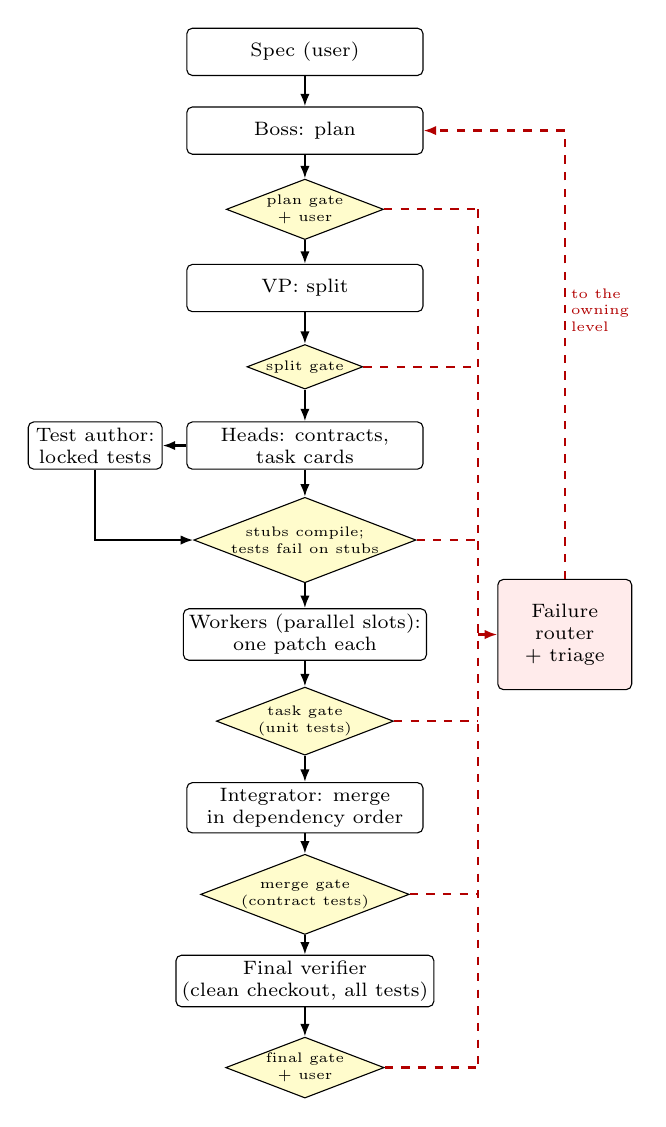
\begin{tikzpicture}[
  font=\scriptsize, x=1mm, y=1mm,
  role/.style={draw, rounded corners=2pt, align=center, minimum width=30mm, minimum height=6mm, inner sep=2pt, fill=white},
  side/.style={draw, rounded corners=2pt, align=center, minimum width=17mm, minimum height=6mm, inner sep=2pt, fill=white},
  chk/.style={draw, diamond, aspect=2.6, inner sep=0.3pt, fill=yellow!20, font=\tiny, align=center},
  arr/.style={-{Latex[length=1.6mm]}, thick},
  back/.style={-{Latex[length=1.6mm]}, thick, dashed, red!70!black},
  busl/.style={thick, dashed, red!70!black},
]
\def\cx{-6}
\node[role] (spec) at (\cx,112) {Spec (user)};
\node[role] (boss) at (\cx,102) {Boss: plan};
\node[chk]  (g1)   at (\cx,92)  {plan gate\\+ user};
\node[role] (vp)   at (\cx,82)  {VP: split};
\node[chk]  (g2)   at (\cx,72)  {split gate};
\node[role] (head) at (\cx,62)  {Heads: contracts,\\task cards};
\node[chk]  (g3)   at (\cx,50)  {stubs compile;\\tests fail on stubs};
\node[role] (w)    at (\cx,38)  {Workers (parallel slots):\\one patch each};
\node[chk]  (g4)   at (\cx,27)  {task gate\\(unit tests)};
\node[role] (int)  at (\cx,16)  {Integrator: merge\\in dependency order};
\node[chk]  (g5)   at (\cx,5)   {merge gate\\(contract tests)};
\node[role] (fin)  at (\cx,-6)  {Final verifier\\(clean checkout, all tests)};
\node[chk]  (g6)   at (\cx,-17) {final gate\\+ user};
\node[side, left=3mm of head] (qa) {Test author:\\locked tests};
\node[side, fill=red!8, minimum height=14mm] (tri) at (27,38) {Failure\\router\\+ triage};
\foreach \a/\b in {spec/boss, boss/g1, g1/vp, vp/g2, g2/head, head/g3, g3/w, w/g4, g4/int, int/g5, g5/fin, fin/g6}
  \draw[arr] (\a) -- (\b);
\draw[arr] (head) -- (qa);
\draw[arr] (qa.south) |- (g3.west);
% failure bus on the right
\draw[busl] (16,92) -- (16,-17);
\foreach \g in {g1,g2,g3,g4,g5,g6}
  \draw[busl] (\g.east) -- (16,0 |- \g.east);
\draw[back] (16,38) -- (tri.west);
\draw[back] (tri.north) |- (boss.east) node[pos=0.3, right, font=\tiny, align=left, xshift=-0.5mm] {to the\\owning\\level};
\end{tikzpicture}
\caption{The company at a glance: work moves down only through a passed gate; every failed gate (diamond) sends its evidence along the dashed bus to one failure router, which returns it to the level that owns it. The user approves at the plan gate and the final gate. The test author's tests are written and locked before any worker starts.}
\label{fig:company}
\end{figure}

\begin{table*}[t]
\caption{Roles in the agent company}
\label{tab:roles}
\centering\footnotesize
\begin{tabularx}{\textwidth}{@{}L{30mm}L{14mm}L{14mm}YYL{26mm}@{}}
\toprule
Role & Kind & Model & Receives & Produces & Checked by \\
\midrule
Boss (planner) & AI & Heavy & Spec, repository map, memory & Plan with testable acceptance criteria; depth tier & Plan gate + user \\
Boss's assistant, pass 1 (plan critic) & AI + code & Reviewer & Spec, plan & Findings with evidence & Rubric checks in code \\
Vice president (splitter) & AI & Heavy & Plan & Departments, milestones, dependency graph & Split gate \\
VP's assistant (split auditor) & Code + AI & Reviewer & Work breakdown & Coverage report & --- \\
Head of department & AI & Heavy & Its slice, repository map & Contracts, task cards, file ownership & Stubs must compile and import \\
Test author (QA head) & AI & Reviewer & Acceptance criteria, contracts & Acceptance and contract tests, then locked & Tests must fail on the stubs \\
Worker & AI & Fast & One task card, its contracts, relevant code & A patch on its own branch & Task gate \\
Department assistant (integrator) & Code + AI & Fast & Worker branches & Merged branch, test report & Merge gate \\
Boss's assistant, pass 2 (final verifier) & Code + AI & Reviewer & Spec, plan, merged diff, all reports & Verdict with evidence & Final gate + user \\
Triage & Code + AI & Heavy & Failure evidence & Which level owns the failure & Routing rules first \\
\bottomrule
\end{tabularx}
\end{table*}

\paragraph{Models} \emph{Heavy} is the main model (a Qwen3-class 35B-A3B MoE). \emph{Fast} is a small coder that fits fully on the GPU (a 9B-class model). \emph{Reviewer} is a model from a different family (gpt-oss-20b~\cite{gptoss}) so that it does not share the maker's blind spots. All three are swappable by drag and drop. Services that are plain code, not agents: scheduler, model manager (router mode), sandbox runner, ledger, git workspace manager, context packer, and project memory.

\subsection{Artifacts and the ledger}

Every handoff is a typed, versioned record in the project ledger (SQLite plus files under \texttt{.hivi/} in the project), so that any agent's input can be rebuilt and any step replayed. Table~\ref{tab:artifacts} lists them with what validates each. The \emph{context packer} builds each role's prompt from the ledger in a fixed order within the role's token budget: role instructions, the specification excerpt, its own record, the contracts it uses, the relevant code (found with the embedding model and reranker), and finally the last failure's evidence. Stable parts come first (P3) so the engine reuses its prompt cache, and the whole prompt fits an 8K--16K context.

\begin{table}[t]
\caption{Artifacts in the project ledger}
\label{tab:artifacts}
\centering\footnotesize
\begin{tabularx}{\columnwidth}{@{}L{17mm}L{16mm}YL{22mm}@{}}
\toprule
Artifact & Written by & Must contain & Validated by \\
\midrule
Spec & User + clarifier & Goal, constraints, out of scope, examples & User approval \\
Plan & Boss & Milestones; acceptance criteria each with a command and expected result; risks; tier & Plan gate \\
Work breakdown & VP & Departments, milestones per department, dependency graph & Every plan item owned exactly once; no cycles \\
Contract & Head & Signatures and types, API schemas, file ownership & Stubs compile and import; no file owned twice \\
Test suite & Test author & Acceptance and contract tests & Fail on stubs first; locked by hash after approval \\
Task card & Head & Goal, files owned, contracts used, tests to pass, budget & Schema \\
Patch & Worker & A diff on its own branch & Applies cleanly; touches only owned files \\
Test report & Sandbox & Command, exit code, failures, log & Produced by code, never by a model \\
Review & Critic or verifier & Findings, each citing a file and line or a test & Rejected if a finding cites no evidence \\
Decision log & Any level & What changed and why & Append-only \\
\bottomrule
\end{tabularx}
\end{table}

\subsection{The main loop}

The loop is a chain of seven steps and five gates with one failure router: work moves down only through a passed gate, and every failed gate sends its evidence to the router. The user approves at two gates (plan and final); the other three are checked by code first, with an AI review on top where code cannot judge.

\subsection{Failure routing and budgets}

A failure goes back to the level that owns it, decided first by \emph{which gate failed} and only then, if the rules cannot tell, by AI triage (Table~\ref{tab:routing}). Default budgets, editable per run: a worker gets three attempts per task; a head two contract revisions per department; the vice president one re-split per milestone; the boss one re-plan per milestone; the whole run has time and token limits set when the user approves the plan. When the top budget runs out, \hivi{} stops and reports what passed, what failed, and the evidence.

\begin{table}[t]
\caption{Failure routing}
\label{tab:routing}
\centering\footnotesize
\begin{tabularx}{\columnwidth}{@{}YL{15mm}Y@{}}
\toprule
What failed & Owner & What happens \\
\midrule
A task's unit tests & Worker & Retry with the error output, up to the worker budget \\
The same error twice in a row & --- & No more retries at that level; escalate one level \\
A patch touches files it does not own & Worker & Rejected without running; retry \\
Workers' branches conflict & Head & Ownership was wrong: fix the contract, re-issue only the affected tasks \\
Contract tests fail after the merge & Head & Revise the contract, re-run dependent tasks \\
Acceptance tests fail while every department passes & VP & The split missed something: re-split that milestone \\
A criterion cannot be tested or contradicts the spec & Boss & Re-plan that milestone \\
The spec is ambiguous & User & One question; only that branch pauses \\
A worker claims a test is wrong & Test author & Reviewed with evidence; a locked test changes only with the user's approval \\
\bottomrule
\end{tabularx}
\end{table}

Three rules stop spinning. \emph{A retry must change its input}: new error output or new context; an identical prompt is never sent twice. \emph{Stall detection}: each failure gets a signature (failing test plus error type) and a repeated signature escalates at once. \emph{Oscillation detection}: if fixing $A$ breaks $B$ and fixing $B$ breaks $A$, the alternating failure sets are recognised and the head re-plans both tasks together. \emph{Recovery}: a checkpoint is saved after every gate (the LangGraph SQLite checkpointer already used in the ProjectRoom), and after a crash the run resumes from the last passed gate.

\subsection{Every known problem and its fix}

Table~\ref{tab:problems} is the design's own checklist: each row is a failure mode observed in agent systems or in the prototype, paired with the mechanism that addresses it. We include it in full because the mapping from problem to mechanism is the substance of the design.

\begin{table}[t]
\caption{Known problems of agent companies and the corresponding mechanism}
\label{tab:problems}
\centering\footnotesize
\begin{tabularx}{\columnwidth}{@{}L{27mm}Y@{}}
\toprule
Problem & Mechanism \\
\midrule
One GPU, many agents & Two or three shared models; work runs in phases; workers share parallel slots of the fast model \\
Model swaps take 20--30~s & Batch by model; router mode keeps the fast model loaded \\
Details lost down the chain & Ledger and context packer; no agent receives a summary of a summary \\
An assistant re-reading with the same blind spots & Checks run code; the reviewer is a different model family; tests are written by another role before the code \\
Workers' pieces do not fit & Contracts and file ownership fixed before splitting; one branch per worker; merges in dependency order \\
Workers gaming the tests & Tests locked by hash; test files off limits to workers; the final check re-runs everything from a clean checkout \\
Endless loops & Budgets per level; stall and oscillation detection; escalation ends with the user \\
A plan that sounds right but is wrong & Every criterion must be testable; plan critic; the user's approval \\
Seven layers for a one-line fix & Depth tiers \\
Made-up APIs or packages & Repository search and documentation lookup; imports checked; packages installed only from the lockfile \\
Context overflow & Token budget per role; retrieval picks only relevant code \\
Malformed agent output & JSON-schema decoding; reject and retry \\
Flaky tests & A failure is re-run twice before anyone is blamed; flaky tests are marked \\
Unsafe generated code & Sandbox: project folder only, no network by default, time and memory limits \\
Crash mid-run & Checkpoint per gate; resume \\
Quality drifting unnoticed & Pass rate and retries tracked per role and shown in the UI \\
\bottomrule
\end{tabularx}
\end{table}

\subsection{Depth tiers}

The boss sizes each request and uses only the levels it needs; the gates are the same at every tier. \emph{T0 Answer}: a question, no code change---one model, normal chat. \emph{T1 Fix}: a clear change to one or two files---worker, test author, final verifier. \emph{T2 Feature}: several files in one area---head, test author, workers, integrator, final verifier. \emph{T3 Project}: several areas or a new application---the full company. The boss estimates from the plan (areas touched, files touched, open unknowns); a run moves up a tier when a split outgrows it, and the user can force a tier.

\subsection{Running it on one 8~GB GPU}

All roles share two or three models and the scheduler runs work in phases so the GPU switches models only between phases: (1) a planning phase on the heavy model (boss, vice president, heads, triage); (2) a review phase on the reviewer model (plan critic, split auditor, test author); (3) a build phase on the fast model, with workers running side by side in \texttt{llama.cpp} parallel slots (each slot gets an equal share of the context); (4) a check phase, code first (sandbox tests, lint, type checks), then the reviewer model for the final review. A failure that goes back up waits for the next phase of its model rather than forcing a swap, unless it blocks everything else. Router mode keeps the fast model loaded between phases when RAM allows while the heavy model swaps in and out. Role instructions never change during a run and the packer puts them first, so the cached prefix is reused. Each model keeps its usual engine rule; parallel worker slots need \texttt{llama.cpp}. The number of slots trades total throughput against per-worker speed and is chosen by measuring on the benchmark suite, not by guessing.

\subsection{Model assignment and the live UI}

The UI is the organisation chart itself. An \emph{org-chart editor}: each role is a node; drag a model card onto it; \hivi{} warns when a model cannot do the job (too little context, no JSON-schema support, too large to share the GPU); saving writes the role configuration file that already exists. A \emph{live run view}: every node shows its state---idle, working, checking, failed, escalated---and a click shows its packed input, its output and its gate results. A \emph{plan approval screen} to read and edit the plan and its acceptance criteria before anything runs. A \emph{workspace}: editor, a diff per worker branch, test reports, the merge view, and a ledger timeline that can be replayed step by step. \emph{Budget meters}: attempts and time used at each level, so a struggling run is visible before it escalates.

\subsection{Build phases and proof}

The company is built from the bottom up, and a phase moves on only when the benchmark suite shows the current one works (Table~\ref{tab:idephases}). The proof is a local suite of about thirty tasks across the tiers---bug fixes, small features, small applications---each with hidden acceptance tests the agents never see, in the manner of SWE-bench~\cite{swebench} at personal scale. Every phase is measured on tasks fully passed on the first run, escalations to the user, retries per level, and wall-clock time per task; a phase ships only if it beats the previous one on that suite.

\begin{table}[t]
\caption{Build phases of the agent company and their exit tests}
\label{tab:idephases}
\centering\footnotesize
\begin{tabularx}{\columnwidth}{@{}L{16mm}YL{24mm}@{}}
\toprule
Phase & What & Exit test \\
\midrule
\phase{IDE-1} Foundations & Artifact schemas, ledger, sandbox runner, context packer, budgets & Unit tests for each service \\
\phase{IDE-2} T1 loop & Worker + locked tests + final verifier, grown from the ProjectRoom (today: one calculator task) & Beats single-shot on the benchmark suite \\
\phase{IDE-3} T2 & Heads with contracts, test author, parallel workers, integrator with git branches & Beats \phase{IDE-2} on multi-file tasks \\
\phase{IDE-4} T3 & Boss, vice president, critics, failure router, triage & Beats \phase{IDE-3} on project-size tasks \\
\phase{IDE-5} UI & Org-chart editor, live run view, plan approval, workspace, budget meters & A full run driven from the UI \\
\phase{IDE-6} Learning & Project memory of failures and fixes per role, fed back through the packer & Fewer retries per level over time \\
\bottomrule
\end{tabularx}
\end{table}

\subsection{Builds on what exists, and prior art}

The role-to-model mapping and automatic swaps (\texttt{model\_roles.yaml}, the model router), the LangGraph generate--test--retry loop with a deterministic test gate and SQLite checkpoints (ProjectRoom), and \texttt{llama.cpp} router mode are the existing pieces the company grows from. MetaGPT~\cite{metagpt} and ChatDev~\cite{chatdev} showed that an LLM ``software company'' works for small applications and that verification and integration are its weak points; the gates, contracts, locked tests and failure routing above are aimed precisely there.

\section{Autonomy: Always-On Operation, Night Shift, Self-Improvement, Desktop Control and Calls}
\label{sec:autonomy}

The features in this section move \hivi{} from a tool the user operates to an agent that works while the user is away. Each is a client of the security base (\sect{sec:security}); together they are the reason that base is built early.

\subsection{Always-on \hivi{} and phone control}

The goal: from the user's phone, anywhere, ``\hivi{}, until I reach home make me $X$, $Y$ and $Z$''---the work happens in the background and is done on arrival; routines run on their own; the assistant messages the user when something needs them.

\paragraph{What is physically possible} A shut-down laptop runs nothing; everything else is possible (Table~\ref{tab:laptop}). The practical set-up is a laptop kept plugged in and set to sleep rather than shut down, with wake-on-network enabled; \hivi{} keeps it awake only while jobs run.

\begin{table}[t]
\caption{What \hivi{} can do in each laptop state}
\label{tab:laptop}
\centering\footnotesize
\begin{tabularx}{\columnwidth}{@{}L{30mm}Y@{}}
\toprule
State & Capability \\
\midrule
On (lid closed is fine, plugged in) & Everything: tasks, routines, messages \\
Asleep & The phone can wake it (Wake-on-LAN; Ethernet best, Wi-Fi depends on the laptop), then it works \\
Shut down & Nothing runs; tasks queue and start the moment it boots \\
Optional later: small always-on box & Holds the queue and wakes the laptop; can run tiny models for quick answers; heavy work waits for the laptop \\
\bottomrule
\end{tabularx}
\end{table}

\paragraph{Phone control} A private connection through Tailscale (a WireGuard~\cite{wireguard} overlay between phone and laptop) so \hivi{} is reachable from anywhere without opening a port to the internet; the web UI as an installable phone app (PWA) with the same chats, memory and models, by text or voice; optionally a Telegram bot linked to the user's account alone; push notifications (``Done: 3 files ready'', ``Needs your OK'', ``Failed: here's why''); and login with device approval (\phase{SEC-3}), because anyone reaching \hivi{} could run code on the laptop.

\paragraph{Background jobs} A SQLite job queue: every task from the phone becomes a job with status (queued, running, needs approval, done, failed), progress and results. Jobs survive a closed browser, lost signal, a crash (resuming from the last checkpoint) and a reboot (\hivi{} starts with the OS as a background service). The runner keeps the laptop awake only while a job runs, uses the same engines as chat (search, agents, image and voice generation), and lands results on the job's page on the phone.

\paragraph{``Almost alive'': routines and watchers} Scheduled routines (``every morning at 8, summarise new data-science job postings''; ``every Sunday, back up my memories''); watchers that check a page, folder or repository on a schedule and act or notify on change; proactive messages only when something matters---a job finished, a watcher fired, an approval is needed---never spam.

\paragraph{Safety} Remote control is power over the laptop, so the phone-side view of the shared gate applies: reading, searching, writing inside the workspace, generating images and voice, and running sandboxed code proceed without asking; deleting or overwriting files outside the workspace, sending or posting anything, and spending, installing or changing system settings need approval on the phone. A kill switch on the phone stops all jobs instantly; the activity log shows everything done while the user was away; per-job budgets (time, model calls) ensure nothing runs forever.

\paragraph{Phases} \phase{LIVE-1}: job queue and background runner, starts with the OS, keep-awake, job status page. \phase{LIVE-2}: phone access (Tailscale, PWA, push). \phase{LIVE-3}: approvals from the phone, kill switch, activity-log viewer. \phase{LIVE-4}: routines and watchers. \phase{LIVE-5}: Telegram bot, voice from the phone. \phase{LIVE-6}: wake from sleep, optional always-on box.

\subsection{Night shift}

While the user sleeps, \hivi{} does the maintenance and heavy work that would slow it down during the day, then leaves a short morning report with anything needing a decision. It runs in a window the user sets (for example 2--6~a.m.), only when plugged in and with normal GPU temperature; the user always wins---starting to use the PC or messaging from the phone pauses night work instantly. The night's job list, in priority order: backup snapshot; health check (disk space, log clean-up, engine self-test); memory tidy (merge duplicates, flag outdated facts for review---never deleting on its own); re-index changed files and rebuild embeddings after an embedding-model change; regression exams on the current models; the model scout (candidates downloaded and examined); every skill's tests, flagging broken ones; research prep (pre-searching topics from tomorrow's open tasks and watched subjects so morning answers are instant); and long jobs the user queued (overnight experiments, agent runs, image batches). Limits: a time, energy and disk budget per night, with checkpoints so a job continues the next night; anything that sends, spends or changes files outside the workspace is not done at night and waits in the morning report. The report is one card in the app and a phone notification: what ran, what failed, backup status, and the decisions waiting (``switch to this model?'', ``merge these 3 memories?'', ``keep this new skill?''), each with one-tap buttons.

\paragraph{Phases} \phase{NIGHT-1}: window, plug-in and temperature checks, pause when active; backups, health checks, re-index; morning report. \phase{NIGHT-2}: memory tidy suggestions, exams and scout, skill tests, research prep, queued long jobs.

\subsection{Self-improvement: models, skills, workflows and blueprints}

Once a day \hivi{} checks whether something better exists---a new model, a better way to do a skill, a better workflow---tests it on the user's own machine, and asks: ``I found $X$; it scored better than what I use now on these tests. Want me to switch?''

\paragraph{The core rule} Nothing changes unless it wins on \hivi{}'s own exams (P7). Public leaderboards do not know the user's hardware, tasks or settings, so every role and department has a \emph{local exam}: a fixed set of tasks with automatic scoring, and a candidate replaces the incumbent only if it scores better here at a speed the user accepts. Table~\ref{tab:exams} lists the exams; \sect{sec:evaluation} returns to them as the paper's evaluation methodology.

\begin{table}[t]
\caption{Local exams}
\label{tab:exams}
\centering\footnotesize
\begin{tabularx}{\columnwidth}{@{}L{19mm}YL{24mm}@{}}
\toprule
Exam & What it tests & Scored by \\
\midrule
Coding & Fix / implement tasks with hidden tests (the agent-company benchmark suite) & Tests pass \\
Planning / reviewing & Plans and reviews checked against known answers & Rubric + code checks \\
Chat and personality & Fixed conversations; tone and honesty rules (\sect{sec:soul}) & Rubric + the user's past thumbs \\
Search answers & Questions with known answers and sources & Correct facts, correct citations \\
Uncensored builds & The user's refusal test set; drift vs.\ the base model & Refusal count; quality kept \\
Images / voice & Fixed prompts; speed and VRAM & The user's side-by-side picks + speed \\
Speed & Tokens/s, time to first token, RAM and VRAM on this PC & Measured \\
\bottomrule
\end{tabularx}
\end{table}

\paragraph{Daily model scout} (1) Scan, as a scheduled routine: new and trending models on Hugging Face, release notes of model families in use, engine updates. (2) Filter to what fits: 32~GB RAM and 8~GB VRAM; MoE with at most about 8B active parameters; no quantisation worse than Q5 for MoE; an acceptable licence; known uploaders; GGUF or safetensors only (no pickle files); uncensored builds only with a measured refusal and divergence report. (3) Shortlist one to three candidates per role from published results. (4) Download overnight within a disk budget and run the exams on idle time. (5) Report: ``Candidate vs.\ current: +12\% coding tests passed, same speed, 3~GB bigger'', with Switch / Try for a week / Skip buttons in the app or on the phone. (6) Switch safely: the old model stays installed; automatic rollback if the new one fails exams again or the user says ``go back''; unused old models are offered for deletion, never deleted silently.

\paragraph{Skills, workflows and blueprints} Skills improve the same way: weekly re-checks of the sources behind each skill; a new version is built beside the old one and must pass the skill's tests and beat it on quality or speed; failures in real use trigger a revision first. Workflows---how \hivi{} does multi-step work: agent pipelines, the search loop, HAIE's sampling rules, prompt templates, retry budgets, the number of worker slots---improve the same way: \hivi{} proposes variants (a different prompt for the test author, four worker slots instead of three, one more search round), runs them on the exams in the background, proposes a winner with evidence, and records why in the decision log. A guardrail: variants may change prompts, settings and model assignments, never the safety rules, approval rules or exam answers.

\paragraph{The user approves every upgrade} Default: ask before every switch. Optional: auto-apply small wins (settings, prompts) and ask only for model and skill swaps. A weekly ``what got better'' summary with exam scores before and after and what was rolled back. One switch pauses all self-improvement.

\paragraph{\hivi{} improves \hivi{}} The assistant points its own agent company at its own repository: it fixes bugs from its error log, speeds up slow parts and adds small features the user asks for---always on a separate copy, always gated by tests, always with approval. Ideas come from repeated errors in the error log and slowdowns in the speed history (\sect{sec:operations}), failed exams, patterns in thumbs-down feedback, and direct requests. The loop: an issue with evidence (log lines, timings) and a proposed fix; work on a separate branch in a separate folder (a git worktree), never on the running \hivi{}; gates---the full test suite, the exams, and a new test that proves the fix; the user's review of summary, diff and test results; apply safely---snapshot, apply, restart, health check; automatic rollback if the health check or exams fail, or on request within 24 hours. A \emph{protected zone} the assistant may propose changes to but never make: the security base (login, approvals, vault, sandbox, activity log), so it cannot loosen its own limits; exam answers and existing tests, which it may add to but never delete or weaken (the gate checks); and the self-improvement rules and the rollback and backup code themselves, so a bad change can always be undone. Limits: one change at a time, small changes only (a set number of files and lines), a few per week; anything bigger becomes a plan for the user to approve first.

\paragraph{Phases} \phase{UP-1}: local exam suites per role and a scoreboard. \phase{UP-2}: daily scout (scan, filter, shortlist, report). \phase{UP-3}: overnight download and exam runs, Switch / Try / Skip, rollback. \phase{UP-4}: skill self-improvement. \phase{UP-5}: workflow and blueprint variants on exams. \phase{UP-6}: engine update checks with regression tests. \phase{SELF-1}: self-coding, read-only (issues with evidence and proposed patches the user applies). \phase{SELF-2}: applies approved fixes under branch, gates, protected zone, backup, rollback. \phase{SELF-3}: small features from requests; optional auto-apply for tiny fixes that pass every gate, with notification.

\subsection{Desktop control}

\hivi{} uses desktop applications the way the user does---a spreadsheet, the file manager, settings, any app---to finish tasks that have no connector or API. The most reliable method is used first: a direct way (connector, shell, application automation, a file library) whenever one exists; the accessibility tree (buttons, menus and fields by name, e.g.\ via pywinauto) for most apps, which is text rather than pixels and works well with small models; and screenshots with the vision model for apps that do not expose their controls, which works almost anywhere but is slower and less reliable.

This is the strictest feature in \hivi{}. Off by default and enabled per task. An app allow-list, never including password managers, banking, security settings or \hivi{}'s own security settings. Watch mode first: every step shown live and needing approval; later only risky steps ask. Stop instantly with a key on the PC and the kill switch on the phone. Screen content is untrusted (P6). It never fights the user for the mouse: it works only when invited or when the user is away, and later in a separate virtual machine so it never touches the user's session. Screenshots stay in the run log only and are deleted after a few days. A procedure that worked is saved as a skill, so next time is faster and more reliable; once \phase{DESK-3} is in place, phone jobs can include ``while I'm out, do $X$ in that app''.

\paragraph{Phases} \phase{DESK-1}: read-only---look at an app (tree plus screenshot) and guide the user step by step. \phase{DESK-2}: actions in allowed apps with approval per step, live view, stop key. \phase{DESK-3}: longer unattended tasks from the phone in a separate virtual machine; procedures saved as skills.

\subsection{Phone calls}

The final stage: \hivi{} calls the user when something urgent comes up, and the user can call \hivi{} and just talk. It builds on voice mode (\sect{sec:capabilities}) and phone control. Three ways to make the call (Table~\ref{tab:calls}); the app call is built first because it is fully private and free and works anywhere with data.

\begin{table}[t]
\caption{Three ways to place a call}
\label{tab:calls}
\centering\footnotesize
\begin{tabularx}{\columnwidth}{@{}L{17mm}YL{22mm}@{}}
\toprule
Way & How it rings & Privacy / cost \\
\midrule
App call (first) & The phone app rings through a high-priority push; audio phone $\leftrightarrow$ laptop over Tailscale (WebRTC) & Fully private, free \\
Private phone line & A SIP app on the phone registered to a small phone server on the laptop (Asterisk / FreeSWITCH) over Tailscale & Private, free; rings like a real call even with the app closed \\
Real phone number & A telephony provider gives \hivi{} a number; call audio streams to the laptop & Not local: the provider carries the audio; number fee plus per-minute cost \\
\bottomrule
\end{tabularx}
\end{table}

\paragraph{\hivi{} calls the user, urgent only} What counts as urgent is set by the user as rules: a job failed that blocks something due today, an approval needed before a deadline, a watcher marked ``call me''. An escalation ladder: notification first, then a call if there is no answer in $N$ minutes and it is urgent. Quiet hours and a do-not-disturb switch with chosen exceptions. A rate limit of a few calls a day, never repeating the same alert. On the call, \hivi{} says why in one sentence; the user can talk it through, approve or deny by voice (``yes, send it'' / ``no, wait till I'm home''), or say ``text me the details''. A missed call leaves a voicemail-style summary.

\paragraph{The user calls \hivi{}} The same voice conversation mode: interrupt, ask anything, give tasks that go into the job queue. The assistant knows the user's memory, running jobs and routines, so ``how's that job going?'' works. The transcript and anything done are saved to the activity log.

\paragraph{Safety and GPU budget} Caller ID can be faked, so on a real phone number \hivi{} asks for a spoken PIN or passphrase before doing anything beyond chatting; app and private-line calls are already tied to the user's devices. Voice approvals follow the phone rules; risky actions are read back and need an explicit ``yes''. The kill switch works by voice. A live call needs speech-to-text, the chat model and text-to-speech at once; a heavy job using the GPU is paused for the call and resumed after.

\paragraph{Phases} \phase{CALL-1}: app call, using voice mode. \phase{CALL-2}: \hivi{} calls the user (urgent rules, ladder, quiet hours, rate limits, missed-call summary). \phase{CALL-3}: voice approvals and voice kill switch. \phase{CALL-4}: private phone line. \phase{CALL-5}: optional real phone number with spoken PIN.

\section{Operations: Health, Hardware Awareness, Quality and Backups}
\label{sec:operations}

\subsection{System health}

The goal is to see at a glance whether \hivi{} is healthy---GPU, memory, models, speed, errors---and, once it runs unattended, to have it fix the common failures itself and report the rest.

\paragraph{What is shown} Hardware: GPU load, VRAM used and free, temperature and power, CPU, RAM, free disk, from \texttt{nvidia-smi} queries and psutil (both already dependencies). Engines: which engine and model are loaded, resident models in router mode, context size, time since start, from the runtime state and the engine's model list. Speed: time to first token and generation tokens/s for every reply, per model, measured by the proxy on every request so that it works identically for both engines. Features: time spent in HAIE, memory recall, web search, file search, image and voice jobs, and error counts, from timers around each feature written to one log. Storage: sizes of memory, chat history, skills and the models folder; age of the last backup. Jobs, later: queue length, running jobs, failures.

The prototype implements the hardware, engine and speed parts (\phase{HEALTH-1}) as a header chip (VRAM, temperature, tokens/s of the last reply, colour-coded by warning level) and a panel. Two implementation points matter for a single-GPU machine. First, probes are split into \emph{fast} (an \texttt{nvidia-smi} query, sampled at most every 1.5~s) and \emph{slow} (engine device enumeration, power-mode APIs, cached for a minute, refreshed in the background), and a request never waits for a slow probe or for a slow \texttt{nvidia-smi}---it is answered from the last reading, with its age, and the chip dims and reports ``not updating'' if readings stop. Second, the process table (which programs hold VRAM) is the slowest call and is refreshed on a side thread every few seconds rather than on every reading. Without these, readings froze under load and the panel appeared broken; the fix was entirely in \emph{when} things are measured, not what.

\paragraph{Error log and speed history} One structured log (JSON lines) for every feature: time, feature, model, what failed, the error, and what \hivi{} did about it; a viewer with filters and a ``copy for bug report'' that bundles the error, settings and recent log lines without chat content; automatic rotation. Tokens/s and time to first token per model are stored per day, so slowdowns after an update, driver change or new model show with the date they started; the same numbers feed the exams, so a ``better'' model that is much slower on the user's hardware is flagged before a switch.

\paragraph{Watchdog and auto-repair} For unattended running (Table~\ref{tab:watchdog}). Every action is written to the error log and the activity log.

\begin{table}[t]
\caption{Watchdog actions}
\label{tab:watchdog}
\centering\footnotesize
\begin{tabularx}{\columnwidth}{@{}L{27mm}Y@{}}
\toprule
Problem & Action \\
\midrule
Engine crashed & Restart with the same model and settings; resume the running job \\
Engine hung (no tokens for too long, health check fails) & Stop, restart, retry the request once \\
Out of GPU memory & Reload with a smaller context or fewer GPU layers (adaptive, like the router's memory margin); log the change \\
Restarted three times in ten minutes & Stop retrying, mark the model unhealthy, fall back to the other engine or a smaller model, notify the user \\
GPU too hot & Pause background jobs until it cools; chat keeps working \\
Disk almost full & Stop writing large outputs, clear caches, warn \\
A feature keeps failing & Turn that feature off for now, say so in chat, keep everything else running \\
\bottomrule
\end{tabularx}
\end{table}

\subsection{Hardware awareness}

When its hardware changes, \hivi{} notices, re-tunes itself, tells the user what it can do now, and never crashes because a setting no longer fits (P9). On every start it reads a hardware fingerprint---GPU model(s) and VRAM, number of GPUs, RAM, CPU, free disk, driver and CUDA version---and compares it with the last start. On an \emph{upgrade} (new GPU, second GPU, more RAM) it re-runs its speed tests, re-tunes context size, GPU layers, how many models stay loaded and the router's memory margin, checks which models now fit, on multi-GPU assigns jobs (chat on one card; voice, images and agent workers on the other), and tells the user in its own voice: ``New GPU: 24~GB. I re-tuned myself. Replies are about $3\times$ faster, and I can now run voice and chat at the same time. Thank you.'' On a \emph{downgrade} (back on the laptop, a GPU removed) it switches to a lighter set-up on its own---smaller context, fewer loaded models, heavy features scaled down---says what is limited for now, and never crashes on load. On a driver or engine update it runs a quick speed test and warns if it got slower. Settings are saved per machine, so moving between a laptop and a home server switches instantly; a hardware timeline records every change with its date, speed before and after, and what became possible; and the model scout then suggests models that only now fit.

\paragraph{Phases} \phase{HEALTH-1} (status panel; implemented), \phase{HEALTH-2} (per-feature timings, error log with viewer, speed history), \phase{HEALTH-3} (watchdog, out-of-memory fallback, heat and disk guards, phone notifications); \phase{HW-1} (fingerprint, re-tune, lighter set-up on downgrade, upgrade/downgrade message), \phase{HW-2} (per-machine profiles, multi-GPU assignment, hardware timeline), \phase{HW-3} (scout suggests newly fitting models; exams re-run after every hardware change).

\subsection{Quality: tests and the QA swarm}

A one-person project has a polish gap. The plan closes it with a swarm of cloud agents (through their APIs) that continuously test, review and fix \hivi{}---the same way the agent company builds software---while the tests themselves run on the user's real hardware.

\paragraph{The test foundation} Unit and integration tests (the existing pytest suite, extended to every section); end-to-end UI tests in which a browser robot (Playwright) uses the application as a user does---send, stream, stop, switch models, attach files, approve actions; GPU tests with real engines and tiny models on every change and real models nightly; a self-hosted test runner so every push runs on the user's PC or home server with a real GPU and real OS, not only in the cloud; and a crash and error reporter that turns repeated errors from the error log into issues automatically---error details only, never chat content.

\paragraph{The swarm} A test writer that finds untested code and writes tests, section by section; a bug hunter for odd inputs, edge cases, fuzzing and cross-feature scenarios (voice mode plus an agent run plus a backup at once); a chaos tester that kills an engine mid-reply, fills the disk, drops the network, exhausts GPU memory, sleeps the laptop; a fixer that takes a confirmed bug to the smallest fix plus a proving test, as a pull request; a reviewer that reviews every change---the user's, the swarm's and \hivi{}'s own self-fixes---using a different model from the one that wrote it; and a release checker that runs the full regression before any model, engine or package update lands. The swarm runs through a coding-agent tool in headless mode in the repository, with keys from the vault.

\paragraph{The loop and the rules} An issue (from the error reporter, a failing test or the bug hunter); reproduce first---a failing test is required, and without a reproduction there is no fix; fix on a separate branch; gates---the full suite on the GPU runner, end-to-end tests, review by a second model; the user merges (optionally, tiny fixes that pass every gate merge automatically with notification); close the issue, and the new test guards against regression. Agents work only through branches and pull requests, never on the main branch. Tests can be added, never deleted or weakened; the gate checks this. No personal data goes to the swarm: test data is synthetic; memory, chats and files stay home. Vault secrets are never shown to agents. Cost is controlled by running review and affected tests on every change but the deep runs only nightly; cheaper models write tests while frontier models review and take hard bugs; a monthly budget with a hard stop and a monthly report of bugs found, bugs fixed and cost. What it cannot replace: real-world use (the error reporter covers part), the user's taste in how things should feel, and hardware it has never seen.

\paragraph{Phases} \phase{QA-1}: end-to-end UI tests, self-hosted runner, error reporter to issues. \phase{QA-2}: cloud swarm with the test writer nightly, the reviewer on every change, budget and report. \phase{QA-3}: bug hunter, chaos tests, fixer with pull requests, release checker. \phase{QA-4}: cross-feature scenario suites for every section; the swarm and \hivi{}-improves-\hivi{} share one issue queue and the same gates.

\subsection{Backups and restore}

Months of memory, skills and settings must not be lost to a dead disk, a bad update or a stolen laptop. Backups run on their own, are encrypted, and restoring is one step.

\paragraph{What is backed up} Personal memory and chat history; the skills folder with versions and tests; settings, engine pins, router presets, HAIE settings; feedback and preference data; agent-company ledgers and blueprints; the job queue, routines and watchers; character adapters and voice references; connector settings, with secrets only inside the encrypted backup. Not backed up: models (re-downloadable; only the list of models, sources and file hashes is saved), caches (rebuilt on use), embedding indexes (rebuilt from the originals), and the user's own files in library folders, which are theirs to back up---\hivi{} stores only the folder list.

\paragraph{How} Consistent copies: SQLite databases are copied with SQLite's online backup, not as raw files, so a backup taken mid-write is never corrupt. Encrypted, incremental, de-duplicated through a tool such as restic~\cite{restic}, with a key derived from the user's passphrase, so daily backups stay small. Destinations: an external drive by default, a second PC or NAS, or a cloud of the user's choice---data is encrypted before it leaves the machine. When: daily, and automatically before risky changes (an update, a model switch, a skill or workflow upgrade, a new adapter, any restore). Retention: 7 daily, 4 weekly and 6 monthly snapshots, adjustable. A recovery key shown once at set-up; without the passphrase or the key nobody can open the backups, including the user.

\paragraph{Restoring and verifying} Everything onto a new PC: install, choose ``restore from backup'', enter the passphrase; memory, skills and settings are back and missing models are downloaded from the saved list. Just one thing: a deleted memory, an older skill version, settings only. A restore-points screen with every snapshot, its date and what changed, with preview. An automatic test restore once a month into a temporary folder with an integrity check; backup age on the health dashboard and a phone notification if the last good backup is older than a few days or the drive is missing; the Markdown memory export kept as a readable copy alongside.

The prototype implements \phase{BAK-1}: a daily local snapshot (memory, chat history, feedback, settings and configuration; models never) to a folder or external drive of the user's choice, ``back up now'', keep-newest-$N$ retention, and one-click restore that first takes a safety snapshot of the current state. \phase{BAK-2}: encrypted incremental backups, cloud destinations, retention rules, recovery key, phone alert. \phase{BAK-3}: restore-points screen, single-item restore, monthly test restores, snapshots before every self-improvement upgrade.

\section{Build Order and Dependencies}
\label{sec:buildorder}

The sections above describe some two dozen areas, each with several phases. The order in which they are built is itself a design decision. Two rules fix it: \emph{finish one stage before starting the next}, and \emph{every stage ends with something the user uses every day}. A third rule, already visible in \sect{sec:security}, places each security phase immediately before the first feature that would need it. Table~\ref{tab:stages} gives the nine stages; Fig.~\ref{fig:deps} gives the dependency graph that produced them.

\begin{table*}[t]
\caption{Build order: nine stages}
\label{tab:stages}
\centering\footnotesize
\begin{tabularx}{\textwidth}{@{}cL{28mm}YY@{}}
\toprule
Stage & Theme & Phases & Why at this point \\
\midrule
1 & Quick wins (days) & Engine pin, real parameter counts, thinking toggle, MTP decoding (\sect{sec:models}); personality and user name (\sect{sec:soul}); \phase{HEALTH-1} status panel, \phase{HW-1} hardware awareness (\sect{sec:operations}); \phase{QA-1} test foundation & Small, low-risk, improves daily use at once. \phase{HEALTH-1} is implemented. \\
2 & She knows you & \phase{MEM-1}--\phase{MEM-3} (and \phase{MEM-4}); \phase{SOUL-1}, \phase{SOUL-2}; \phase{BAK-1} & Memory and mood awareness are what every later feature (voice, phone, calls) relies on; backups start the day there is memory worth losing. Implemented. \\
3 & She can look things up & \phase{SEC-1}; \phase{CLOUD-1}; \phase{QA-2}; search phase 1 (1.1--1.9); \phase{FILE-1}, \phase{FILE-2}; \phase{PROJ-1} & Security base first: from here on \hivi{} reads untrusted content. Skills, deep research and self-improvement all need search; files reuse the same pipeline; projects group chats, files and instructions; cloud keys need the vault. \\
4 & She can make things & \phase{SEC-2} sandbox; \phase{CLOUD-2}; \phase{SKILL-1}, \phase{SKILL-2}; \phase{CODE-1}, \phase{CODE-2}; \phase{CANVAS-1}, \phase{CANVAS-2}; \phase{MCP-1}, \phase{MCP-2}; \phase{IMG-1}, \phase{IMG-2}; \phase{VOX-1}, \phase{VOX-2} & Sandbox before running skill code; the skills format first so images and voice ship as skills; the code interpreter and canvas reuse the sandbox; connectors give her hands. The biggest stage---split if it drags. \\
5 & She can talk & \phase{TALK-1}--\phase{TALK-3}; \phase{VOX-3}; \phase{PRES-2} & Needs speech-to-text and voices from stage 4. \\
6 & She builds software & \phase{UP-1} exams; \phase{IDE-1}--\phase{IDE-5}; \phase{MCP-3}; \phase{HEALTH-2}; \phase{PROJ-2}; \phase{CLOUD-3}; \phase{QA-3} & The biggest build; the exams double as the benchmark; timings and error logs make long runs debuggable. \\
7 & She works while you're away & \phase{SEC-3} login and encryption first; \phase{HEALTH-3} watchdog; \phase{BAK-2}; \phase{LIVE-1}--\phase{LIVE-5}; \phase{MCP-4}; \phase{NIGHT-1}; \phase{HW-2} & Login before the phone can reach her; watchdog and backups before she runs unattended; then agent runs, images and research become background jobs started from the phone. \\
8 & She learns and improves & \phase{SKILL-3}--\phase{SKILL-5}; search phase 2; \phase{SOUL-3}, \phase{SOUL-4}; \phase{MEM-5}; \phase{IDE-6}; \phase{UP-2}--\phase{UP-6}; \phase{IMG-3}, \phase{IMG-4}; \phase{FILE-3}; \phase{MCP-5}; \phase{BAK-3}; \phase{PROJ-3}; \phase{CODE-3}; \phase{CANVAS-3}; \phase{NIGHT-2}; \phase{SELF-1}, \phase{SELF-2}; \phase{DESK-1}, \phase{DESK-2}; \phase{CLOUD-4}; \phase{HW-3}; \phase{QA-4} & Needs search, skills, exams and background jobs all in place. \\
9 & She calls you (final) & \phase{CALL-1}--\phase{CALL-5}; \phase{LIVE-6}; \phase{SOUL-5}; \phase{TALK-4}; \phase{SEC-4}; \phase{SELF-3}; \phase{DESK-3}; \phase{PRES-3} & Builds on voice mode, phone control and everything before it. \\
\bottomrule
\end{tabularx}
\end{table*}

\begin{figure*}[t]
\centering
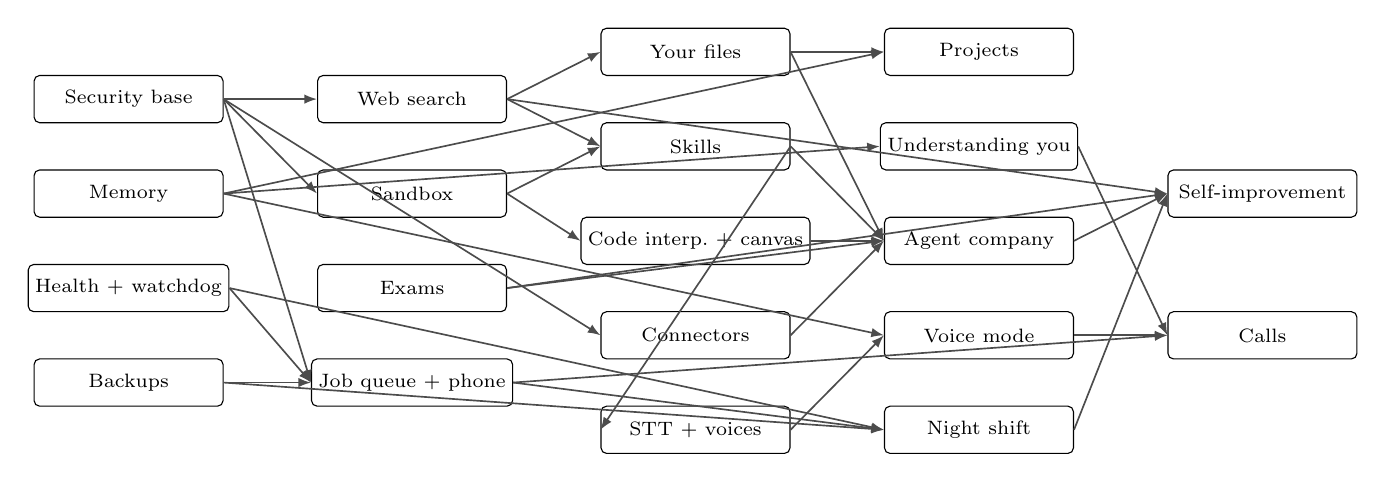
\begin{tikzpicture}[
  font=\scriptsize, x=1mm, y=1mm,
  n/.style={draw, rounded corners=2pt, align=center, inner sep=2.5pt, minimum height=6mm, minimum width=24mm, fill=white},
  arr/.style={-{Latex[length=1.6mm]}, semithick, gray!60!black, rounded corners=2pt},
]
% layer 1
\node[n] (sec)    at (0,30)  {Security base};
\node[n] (mem)    at (0,18)  {Memory};
\node[n] (health) at (0,6)   {Health + watchdog};
\node[n] (bak)    at (0,-6)  {Backups};
% layer 2
\node[n] (search) at (36,30) {Web search};
\node[n] (sand)   at (36,18) {Sandbox};
\node[n] (exams)  at (36,6)  {Exams};
\node[n] (live)   at (36,-6) {Job queue + phone};
% layer 3
\node[n] (files)  at (72,36) {Your files};
\node[n] (skills) at (72,24) {Skills};
\node[n] (code)   at (72,12) {Code interp.\ + canvas};
\node[n] (mcp)    at (72,0)  {Connectors};
\node[n] (vox)    at (72,-12){STT + voices};
% layer 4
\node[n] (proj)   at (108,36){Projects};
\node[n] (soul)   at (108,24){Understanding you};
\node[n] (ide)    at (108,12){Agent company};
\node[n] (talk)   at (108,0) {Voice mode};
\node[n] (night)  at (108,-12){Night shift};
% layer 5
\node[n] (self)   at (144,18){Self-improvement};
\node[n] (calls)  at (144,0) {Calls};
\foreach \a/\b in {sec/search, sec/sand, sec/live, mem/soul, mem/proj, health/live, bak/live, health/night, bak/night,
  search/files, search/skills, sand/code, sand/skills, exams/ide, live/night, live/calls,
  files/proj, files/ide, skills/vox, skills/ide, code/ide, mcp/ide, vox/talk, mem/talk,
  talk/calls, ide/self, exams/self, search/self, night/self, soul/calls, sec/mcp}
  \draw[arr] (\a.east) -- (\b.west);
\end{tikzpicture}
\caption{Dependencies at a glance, read left to right (an arrow means ``is needed by''). The security base feeds every feature that reads untrusted content or acts; memory feeds understanding, voice mode and calls; the search pipeline feeds files, skills and self-improvement; exams feed the agent company and all upgrades; the job queue with the watchdog and backups feeds unattended running.}
\label{fig:deps}
\end{figure*}

\paragraph{Dependencies in words} Memory is needed by understanding the user, voice mode and calls. Web search is needed by skills, deep research and self-improvement. Skills are needed by images, voice and agent workers. Speech-to-text and voices are needed by voice mode, which is needed by calls. Exams are needed by the agent-company benchmark, which is needed by model, skill and workflow upgrades. The job queue and login are needed by phone control, which is needed by calls. The security base is needed by skills, connectors, the agent company, phone control and calls. Watchdog and backups are needed by unattended running. The search pipeline is needed by files, which are needed by the psychology library and the agent company's code index. Connectors are needed by agent tools and by phone jobs on calendar and email. The sandbox is needed by the code interpreter, which is needed by the code canvas and spreadsheet questions. Memory and files are needed by projects, which are needed by agent projects. The job queue, watchdog and backups are needed by night shift. The agent company, exams, backups and the security base are needed by \hivi{}-improves-\hivi{}. The security base and vision are needed by desktop control. The secrets vault is needed by cloud models, which are needed by escalation, cloud agent roles and the QA swarm. Hardware awareness means every feature gets settings that fit the machine it is on.

\paragraph{Status} Stages 1 and 2 are implemented in the prototype except for the engine-layer items and \phase{QA-1}; the ``animated presence'' phases (\phase{PRES-1} in stage 1, a living visual in the header showing idle, listening, thinking, working, speaking and needs-you states) were dropped from the plan in favour of the brand's static mark and a splash animation, and \phase{PRES-2}/\phase{PRES-3} remain optional.

\section{Evaluation Plan and Early Measurements}
\label{sec:evaluation}

A vision paper owes its readers a statement of how its claims will be tested. \hivi{}'s evaluation has an unusual property that follows from its premise: because the system runs on one person's hardware for one person's tasks, the relevant benchmark is \emph{local}. The exams of \sect{sec:autonomy} are therefore both a feature and the paper's methodology.

\subsection{Local exams as the unit of evidence}

Each role and feature has an exam: a fixed set of tasks with automatic scoring, run on the owner's machine (Table~\ref{tab:exams}). The exams serve three purposes. They gate every change (P7): no model, skill, workflow or self-written patch is applied unless it wins. They are the benchmark for the agent company (\sect{sec:ide}): a suite of about thirty coding tasks across the depth tiers with hidden acceptance tests, measured on first-run pass rate, escalations to the user, retries per level and wall-clock time, with each build phase required to beat the previous one. And they make the hardware-awareness claims testable: after any hardware, driver or engine change the speed exam is re-run and the before/after numbers are recorded in the hardware timeline.

Public leaderboards are used only to shortlist candidates for the scout; they do not decide anything, because they do not know the user's hardware, quantisation, context budget or tasks.

\subsection{Measurements the prototype already reports}

The prototype measures and stores, for every reply, time to first token and generation tokens per second, server-reported where the engine provides timings and estimated otherwise, per model and engine; model switch timings broken down into wait, stop and load; and GPU readings sampled live. Table~\ref{tab:early} gives representative figures from the target machine during development. They are reported to characterise the regime the design targets, not as a comparative evaluation: the development laptop ran a Qwen3-class 35B-A3B MoE at Q5 quantisation on an 8~GB GPU with CPU offload of experts, and project-memory retains through Hindsight.

\begin{table}[t]
\caption{Representative measurements on the target machine (RTX~5060 laptop GPU, 8~GB VRAM, 32~GB RAM). Characterisation of the regime, not a comparative benchmark.}
\label{tab:early}
\centering\footnotesize
\begin{tabularx}{\columnwidth}{@{}YL{30mm}@{}}
\toprule
Quantity & Value \\
\midrule
Project-memory retain (Hindsight, LLM extraction), short document & $\sim$90--110~s (109~s measured) \\
Cold switch to a $\sim$20~GB MoE model & tens of seconds (20--30~s class) \\
Resident RAM, 35B-A3B chat model plus both CPU side services & $\sim$25~GB before context caches \\
Side-service footprint (embedding, reranker, CPU) & $\sim$2.3~GB each \\
HAIE rule-based classification & negligible (no model call) \\
Health probe cadence & fast every 1.5~s; slow cached 60~s; never on the reply path \\
Personal-memory extraction & one small model call after the reply, cancelled by the next message \\
\bottomrule
\end{tabularx}
\end{table}

Two of these numbers are the direct cause of design decisions. The 109~s retain is why personal memory has its own store and why automatic extraction is a short, schema-checked pass rather than a Hindsight retain. The tens-of-seconds model switch is why the agent company batches work by model and why router mode keeps a fast model resident.

\subsection{Planned experiments}

For each stage the following measurements are planned, with the prototype's test suites extended accordingly.
\begin{itemize}
\item \textbf{Memory (stage 2).} Precision of automatic extraction (fraction of saved facts the user keeps after a week, measured by undo and delete rates); recall quality (fraction of messages where recalled memories were used in the reply, judged by rubric); reply latency with memory on versus off, which the design predicts to be unchanged apart from a few hundred tokens of prompt.
\item \textbf{Mood (stage 2).} Agreement of the rule-based reader with user self-report on a held-out set of messages in English and Hinglish; later, the same for a small learned classifier.
\item \textbf{Search and files (stage 3).} Answer correctness and citation support on a question set with known answers; the fraction of cited sentences the citation check confirms; end-to-end time for quick search (target 5--10~s before generation).
\item \textbf{Agent company (stage 6).} The thirty-task suite as above; the effect of slot count on throughput and per-worker latency; retries per level over time once \phase{IDE-6} learning is in place.
\item \textbf{Self-improvement (stage 8).} Number of scout candidates examined, fraction accepted, fraction rolled back; exam score before and after each accepted switch.
\item \textbf{Security.} A red-team set of prompt-injection attempts through web pages, files and tool results, scored on whether any send, delete or spend action was taken without approval (the design's target is zero).
\end{itemize}

\subsection{Engineering tests}

The prototype carries automated tests for the chat server, HAIE, routers, health probes, personal memory, mood, backups and the desktop launcher (over 140 at the time of writing), plus a browser-driven check of the UI across window widths and themes. The QA plan (\sect{sec:operations}) extends these to end-to-end UI tests on a self-hosted GPU runner.

\section{Limitations, Risks and Open Questions}
\label{sec:limitations}

\subsection{What a single-GPU assistant will not do as well}

\paragraph{Judgment on hard problems} A 35B-A3B MoE at Q5 is not a frontier model. On difficult analysis, conflicting sources and subtle code, it will make more mistakes than a cloud model, and no amount of pipeline design changes that. The design's answers are structural---citation checks, code-run gates, a reviewer from a different family, exams---and, where the user permits, governed escalation to a cloud model (\sect{sec:models}). We think this is the right trade for a personal assistant, but it is a trade.

\paragraph{Latency of multi-step work} Deep research takes minutes, an agent-company run takes longer, and both pause other GPU work. Night shift and background jobs exist because of this; they do not remove it.

\paragraph{Small models and tools} Small models misuse tools, drift from schemas, and over-call. The tool router, constrained decoding and step budgets reduce but do not eliminate this; the plan builds fixed pipelines first and model-decided tool calling later for that reason.

\paragraph{Fine-tuning on 8~GB} Character adapters are limited to small models; the companion-model route gives the character to voice mode but not to the main model.

\subsection{Risks the design creates}

\paragraph{Self-modification} An assistant that edits its own code is a new attack surface. The protected zone, the gate that checks that tests are never weakened, the requirement of a proving test, the backup-before-apply rule and automatic rollback are the mitigations; the user's approval of every change is the backstop. We do not claim the loop is safe in the abstract, only that its failure modes are enumerated and each has a mechanism.

\paragraph{Remote access} Phone control makes the laptop reachable. The overlay network, login with device approval, the kill switch and the approval gate on all state-changing actions are the mitigations, and \phase{SEC-3} precedes \phase{LIVE-2} in the build order for that reason.

\paragraph{Prompt injection} \hivi{} will read web pages, files, emails, tool results and screens. The untrusted-content rule, with its ``always ask while such content is present'' clause, is a policy that works only if every content path is tagged; a missed path is a vulnerability. The red-team experiment in \sect{sec:evaluation} targets this.

\paragraph{Memory errors} Automatic extraction will sometimes save a wrong or unwanted fact. Undo, the management screen, calibration rules and the never-stored list limit the damage; they do not make the extractor correct.

\paragraph{Emotional design} Mood-aware styling and a defined character could, if done badly, encourage dependence. The loyalty rules are written to push the other way, and mood readings are not stored by default. Whether the rules hold in practice is an empirical question for the chat-and-personality exam and for the user.

\paragraph{Uncensored model builds} The prototype supports ``abliterated'' builds and retries with thinking on when such a build refuses. This is the user's choice on their own machine; the design treats it as a configuration, measures refusal and quality drift in the exams, and does not otherwise take a position.

\subsection{Open questions}

How much of the character can be carried by prompt and retrieval alone, before fine-tuning is worth its cost? What is the right default budget for the agent company's loops, and does \phase{IDE-6} learning reduce retries in practice? Can a rule-based mood reader be good enough that a learned one is unnecessary? Does the exam-gated upgrade rule keep pace with model releases, or does it make the assistant conservative? And, most broadly: as unified-memory consumer machines and larger consumer GPUs arrive, which of these designs are permanent and which are artefacts of 8~GB?

\subsection{Threats to validity}

This paper reports a design and a prototype built by a small team for one user on one machine. The measurements in \sect{sec:evaluation} are characterisations, not controlled comparisons. The feature list mirrors commercial assistants and is therefore not independent evidence that those features are the right ones. Several components rely on third-party open-source projects whose behaviour and licences may change.

\section{Conclusion}
\label{sec:conclusion}

We have argued that a personal AI assistant can be built local-first on a consumer machine, and that doing so is a design problem in its own right rather than a scaled-down copy of the cloud. The constraints---one small GPU shared by several models, latency paid directly by one user, the assistant living next to the user's own files and credentials, and hardware that changes over time---reshape every feature. The result is an architecture organised around nine principles: local by default with governed cloud use; nothing model-based on the reply path that can run after it; stable prompt prefixes; execution over opinion; one approval model; untrusted content as data; measured and reversible change; honest, loyal, non-dependent behaviour; and hardware as an input.

The design covers the full feature set users now expect---memory, history, projects, search with citations, files, skills, a code interpreter, a canvas, connectors, images, voice---and goes beyond it to an agent company that produces tested code on one GPU, to always-on operation controlled from a phone, to self-improvement gated by local exams, and finally to calls. Each piece is specified against an 8~GB budget with its failure modes named and a staged plan with exit criteria; a build order of nine stages puts security before exposure and ends every stage with something used daily. A prototype implements the foundation and the first two stages.

What we hope readers take from this is less the feature list than the method: write down the hardware budget, put the security base before the capability that needs it, decide for every feature who holds the GPU when, and refuse to apply any change the system cannot prove on its owner's own machine. We believe this method generalises beyond \hivi{} to any assistant that is meant to be owned rather than rented.


\appendices
\section{Hardware Plan}
\label{app:hardware}

The design above targets an 8~GB laptop GPU. This appendix records the machine the design is meant to grow into, because several components (multi-GPU job assignment, per-machine profiles, the model scout's ``what now fits'') exist for that growth. Prices are rough U.S.\ estimates from November~2026, during a period of elevated memory prices, and should be checked before buying.

\paragraph{The rule} GPU memory---size and speed---decides which models fit, how fast replies come, and whether chat, voice, images and agent workers can run at once. \hivi{} is built on NVIDIA CUDA and Windows (\texttt{llama.cpp}, Colibr\`i), so staying on NVIDIA means nothing needs porting.

\paragraph{The target: a home server} A desktop that stays on all the time; the laptop becomes a screen and a travel machine. Two GPUs rather than one large one, so that chat runs on one card and voice, images and agent workers on the other (Table~\ref{tab:hw}).

\begin{table}[h]
\caption{Target build}
\label{tab:hw}
\centering\footnotesize
\begin{tabularx}{\columnwidth}{@{}L{18mm}YL{19mm}@{}}
\toprule
Part & Pick & Approx.\ cost \\
\midrule
GPUs & $2\times$ used RTX~3090 24~GB (48~GB total) & $\sim$\$2,300 \\
CPU & AMD Ryzen~9 9950X & $\sim$\$550 \\
Motherboard & X870E with two GPU slots at x8/x8 & $\sim$\$450 \\
RAM & 128~GB DDR5 ($2\times64$~GB; speed matters little) & $\sim$\$1,900 \\
Power supply & 1600~W, ATX~3.1 & $\sim$\$400 \\
Case + cooler & High airflow, fits two 3-slot cards & $\sim$\$300 \\
Storage & 4~TB NVMe for models & $\sim$\$500 \\
UPS & 1500~VA, so a power cut does not kill jobs & $\sim$\$250 \\
\midrule
Total & & $\approx$\$6,650 ($\approx$\$5,500 with 64~GB RAM) \\
\bottomrule
\end{tabularx}
\end{table}

\paragraph{Buy it in steps} Step~1: the build above with one 3090 and 64~GB RAM (running total $\sim$\$4,400): three times the GPU memory and an always-on server. Step~2: a second 3090 ($\sim$\$5,500): chat and voice, images or agent work at the same time. Step~3: RAM to 128~GB when prices drop ($\sim$\$6,650): larger MoE models with CPU offload. Later: RTX~5090 or 24~GB ``Super'' cards once prices are near list. The power supply, board and case are chosen so each step drops in without replacing anything. Undervolt the 3090s (20--30\% less power and heat for little speed lost) and check used cards' memory temperatures. Each step triggers hardware awareness (\sect{sec:operations}).

\paragraph{Not now} RTX~5090: street prices several times its list price. RTX~PRO~6000 (96~GB): the ideal card, at a list price around \$16,000. 128~GB unified-memory boxes (DGX~Spark, Strix~Halo mini-PCs, Mac~Studio): run very large models but more slowly, and AMD and Mac would need porting.


\balance
\bibliographystyle{IEEEtran}
\bibliography{refs}

\end{document}
